% ============================================================
%  第五卷 第九章 溶液（§85–§100）
%  底本：高教社中文版第5版（束仁贵/束莼 译，郑伟谋 校）；
%  OCR 底稿 full_merged.md 行 9261–10541
%  插图 30 幅：图20—图30（§97）、图31—图40（§98）、图41（§99，多面板合一）、
%  图42—图49（§100）；无表格。
%  正文圈码 12 处已全部转录为 \footnote{...}（圈码已删；对照原书 pages300
%  p249/p253/p254/p255/p257/p259/p264/p267/p272/p274/p275 逐一核验）：
%  §87 p249①；§89 p253①；§90 p254①②（②在习题1）、p255①（习题2）；
%  §91 p257①（等容类似公式 (91.4a)，即排版代理删除的窜入公式，已按 p257
%  页脚归位，用 \tag{91.4a} 手工编号）；§92 p259①；§94 p264①；
%  §96 p267①（dE_0 微分式，即排版代理删除的窜入公式，已按 p267 页脚归位）；
%  §97 p272①；§98 p274①、p275①。
%
%  已修正的 OCR/原书错误（除注明外均对照 原书转换/pages/ 核验）：
%   [§85] dΦ 展开式中 \frac{d}{dt}×2→\sum_i（OCR 乱码）；"化学势μ—…—
%         粒子数 μ_i N_i 的导数"语序按 p247 复原为"化学势 μ_i——热力学势对
%         组分粒子数 N_i 的导数"；μ_i:=→μ_i=；(85.3)"\sharp…\langle|"→常数；
%         \mathscr{Q}→\varOmega；\phi→\varPhi 全章统一；
%   [§86] (86.1) 末列 μ^r（OCR 作 μ'、\mu_n^1）；"方程组(84.1)"→(86.1)
%         （p247—248，OCR 误抄节号）；
%   [§87] "除以 n!\mathbb{D}"→n!①（圈码误读）；\alpha(P,T,N)（OCR 缺 N）；
%   [§88] "P_2-P_1=\Delta P C 即渗透压"→\Delta P（即渗透压）；
%   [§89] (89.1) 第二个 μ_0^I→μ_0^{II}；展开式与(89.3)(89.4)中罗马数字角标
%         全坏（c_I、c_{II}、v_I、v_{II}、s_I、s_{II}、(s_{II}-s_I)T=q）按
%         p251—252 还原；(89.8) 后"Pv=T、P\approx P_0"两处 υ→v；
%         T_\mathfrak{d}→T_0、\mu_\circ→\mu_0；
%   [§90] "c_t 和 c_2"→c_1 和 c_2；(90.3)"P×\frac{24}{11}-\frac{34}{11}x"→
%         P×常数（p254 原书如此）；习题1"TInc"→T ln c；习题2 关系①
%         （\mathfrak{D}）；"δc_{01}<<c_{01} 5δc_{02}"→≪c_{01}，δc_{02}；
%         (1)式中 \beta_{i1}→\beta_{11}；
%   [§91] δ 系被 OCR 作 8/\S/\mathfrak{s}/\hbar 者一律还原（δΦ、δn、δV、
%         δQ_P 十余处）；"热效应、首先"→热效应.首先（p256）；"R_min=Φ_2-𝒫_1"
%         →Φ_1；\upsilon′→v′；习题1 前 OCR 窜入的公式(91.4a)系 p257 脚注①
%         之内容（"等容过程中热量吸收的类似公式"），删除，脚注文本归脚注代理；
%   [§92] ∫e^{-F(p,q)/T}dT→d\varGamma（p259）；(92.4) 末尾",1^{1/2}"→
%         v^{1/2}（导数分母 ε^{3/2}T^{3/2}v^{1/2}）；ν_o→ν_a、μ_*→μ_s、
%         n_o→n_a；习题(1)(2)编号系原书习题内编号，自动编号无法产生，
%         按 ch04 (42.5a) 先例用 \tag 排；
%   [§93] (93.2) 第二项"=N_2f_2'(T)"→-N_2f_2'(T)（p261）；(93.5) 第二行
%         OCR 全毁，按 p261 还原为 N_1(T\ln P+χ_1)+N_2(T\ln P+χ_2)+…；
%         N_t→N_1、Δs→ΔS；同种气体合并后的熵式无因子 e，原书 p262 如此，照排；
%   [§94] "阶乘之积 N_1:N_2!"→N_1!N_2!；μ_{ci}→μ_{cl}；
%   [§95] 上标 8/∘/s/*→g 或 *：μ_1^g、μ_2^g、w_1^g（蒸气）、w_1^l（液态）、
%         溶液量上标 *（N_1^*、S^*、V^*、Φ^*、W^*）；P_{10}、w_1^1→w_1^l；
%   [§96] OCR 正文窜入的"dE_0=T_0dS_0-P_0dV_0+μ_0'dn_0"系 p267 脚注①之内容，
%         删除，脚注文本归脚注代理；"{\bar H}1"→和；C_\nu→C_v（小写下标，
%         与卷5成品一致）；(96.6)(96.7)(96.8)(96.9) 下标 P,τ→P,T；
%   [§97] μ(P,T,x+8x)→x+\delta x；"∇_μ μ^μ_μ"→μ（OCR 乱码，p269）；
%   [§98] T_4,T_8,T_c（§100）→T_A,T_B,T_C；
%   [全章] \mathrm{d} 收紧；\ln、\exp 函数名统一；υ（upsilon）→v 数十处；
%         中文粘连/断行多处修复；圈码 ①② 与 \mathbb{D}、\mathfrak{D} 之误读还原。
%  遗留问题：
%   - §85"仅在此时上式不再适用"、§87"它应该形为"、§87 首句"我们在§87—§91中"
%     均原书 p247—248 如此，照排；
%   - §89"这个公式给出溶剂饱和蒸气压溶液上方值(P)和纯溶剂上方值(P_0)之差"
%     原书 p253 语序如此，照排；
%   - §83 称"将在§153中研究"、§96 称"与下面在§152中……做法一样"，两处节号
%     不一致系原书 p244/p269 原貌，照排；
%   - §93 同种气体合并后熵式缺因子 e（p262 原书如此），照排；
%   - §98 区域记号"区域 ADB 和 CBE（图35）以及区域 ADB 和 CDE（图36）"之
%     图36 第二区域 CDE 照 OCR（未逐字核页）。
% ============================================================
\chapter{溶液}

\section{由不同粒子构成的系统}

直到现在为止我们还只限于讨论由相同粒子所构成的系统.现在我们要来研究由不同粒子构成的系统.由几种物质混合而成的任何类型的混合物都是这样的系统；如果混合物有一种物质比其它几种多得多，那么它就称为其它几种物质在这种占优势的物质（溶剂）中的溶液.

一些物质在完全平衡时的数量可以任意给定，它们的种数通常称为系统的独立组分的数目.在完全平衡的状态下系统的所有热力学量完全由温度和压强的数值以及独立组分的粒子数来确定.如果系统中不同物质之间可以产生化学反应，那么独立组分的数目可以与系统中不同物质的总数不一致；如果这样的系统处于非完全平衡的状态，那么要确定它的热力学量，一般来讲必须知道系统中所有物质的数量.

可以很容易把§24的结果推广到由不同粒子构成的物体上去.首先，所有的热力学量必须是所有可加性变量——例如各种粒子的数目和体积——的一次齐次函数.

其次，原先作为某个热力学势对粒子数的导数给出物体单一化学势的概念（§24），现在混合物的每种组分有化学势 $\mu_i$——热力学势对组分粒子数 $N_i$ 的导数.相应地，(24.5)，(24.7)—(24.9)所有各式中的 $\mu\mathrm{d}N$ 这一项现在必须代之以和式 $\sum\mu_i\mathrm{d}N_i$.

这样，微分表达式 $\mathrm{d}\Phi$ 写成
\begin{equation*}
  \mathrm{d}\Phi=-S\,\mathrm{d}T+V\,\mathrm{d}P+\sum_i\mu_i\mathrm{d}N_i,
\end{equation*}
而化学势
\begin{equation}
  \mu_i=\left(\frac{\partial\Phi}{\partial N_i}\right)_{P,T}.
\end{equation}
这时化学势被表示为压强、温度和各种物质的浓度（即粒子数之比）的函数.粒子数只能以比值的形式包含在 $\mu_i$ 中，这是因为：$\Phi$ 是 $N_i$ 的一次齐次函数，所以化学势必然是这些变量的零次齐次函数.

根据 $\Phi$ 是 $N_i$ 的一次齐次函数这一事实，从欧拉定理得出：
\begin{equation}
  \Phi=\sum_iN_i\frac{\partial\Phi}{\partial N_i}=\sum_i\mu_iN_i,
\end{equation}
这是公式 $\varPhi=N\mu$ 的推广.

对于热力学势 $\varOmega$，我们现在得到
\begin{equation*}
  \varOmega=F-\sum\mu_iN_i,
\end{equation*}
由此再一次得到公式 $\varOmega=-PV$.如果物体处于外场中而不同部分的压强不同，仅在此时上式不再适用.

§25的结果也可以直接推广：系统在外场中的平衡条件要求每一种组分的化学势都像温度一样在整个系统中都是常数：
\begin{equation}
  \mu_i=\text{常数}.
\end{equation}
最后，由不同粒子组成的系统的吉布斯分布具有形式
\begin{equation}
  w_{nN_1N_2\cdots}
  =\exp\frac{\varOmega+\sum\mu_iN_i-E_{nN_1N_2\cdots}}{T},
\end{equation}
这是公式(35.2)的自然的推广.

\section{相律}

现在我们考虑系统由不同物质构成并形成 $r$ 个相互接触的相（每一相一般来讲包含所有的物质）.

设系统中独立组分的数目为 $n$.于是每一相由压强、温度和 $n$ 个化学势来表征.我们由§81知道：由相同粒子构成的各相的平衡条件是温度相等、压强相等和化学势相等.显然，在有几种组分存在的普遍情形下，各相的平衡条件是温度相等、压强相等和每一个化学势相等.设在所有各相中的共同温度和压强是 $T$ 和 $P$；为了区别属于不同相和不同组分的化学势，我们用两个角标来标记它们：上角标（罗马数字）代表相，下角标（阿拉伯数字）代表组分.于是相平衡条件可以写成形式
\begin{equation}
\begin{aligned}
  \mu_1^{\mathrm{I}}&=\mu_1^{\mathrm{II}}=\cdots=\mu_1^{r},\\
  \mu_2^{\mathrm{I}}&=\mu_2^{\mathrm{II}}=\cdots=\mu_2^{r},\\
  &\cdots\cdots\cdots\cdots\cdots\cdots\\
  \mu_n^{\mathrm{I}}&=\mu_n^{\mathrm{II}}=\cdots=\mu_n^{r}.
\end{aligned}
\end{equation}
这些化学势作为函数每一个都有 $n+1$ 个独立变量：$P$，$T$ 和各种组分在某相中的 $n-1$ 个浓度（每相有 $n$ 个独立的不同种粒子数，它们之间有 $n-1$ 个独立的比值）.

条件(86.1)是一组 $n(r-1)$ 个方程式.这些方程式中的未知数的数目等于 $2+r(n-1)$.这些方程式要有解，它们的数目在任何情况下都必须不大于未知数的数目，即
\begin{equation*}
  n(r-1)\leqslant2+r(n-1),
\end{equation*}
亦即
\begin{equation}
  r\leqslant n+2.
\end{equation}
换句话说，在由 $n$ 种独立组分所构成的系统中，可以有不多于 $n+2$ 个的相同时处于平衡.这就是所谓吉布斯相律.在§81中我们已经有过这个相律的特殊情形：在一种组分的情形下，能够相互接触而同时存在的相的数目不可能大于3.

如果同时共存的相数 $r$ 小于 $n+2$，那么在方程组(86.1)中，有 $n+2-r$ 个变量显然可以具有任意值.换句话说，可以任意改变任何 $n+2-r$ 个变量，而不破坏平衡；当然，同时其余的变量是以完全确定的方式变化的.可以任意被改变而不破坏平衡的变量的数目，称为系统的热力学自由度的数目.如果用字母 $f$ 来代表它，那么就可以把相律写成形式
\begin{equation}
  f=n+2-r,
\end{equation}
式中 $f$ 当然不能小于0.如果相数等于它的最大可能值 $n+2$，那么 $f=0$，这就是说，在方程组(86.1)中所有的变量都是确定的，其中没有一个能够改变而不使平衡破坏或不使任何一相消失.

\section{稀溶液}

我们在§87—§91中要研究稀溶液的热力学性质，所谓稀溶液就是这样的溶液：其中溶质的分子数远远小于溶剂的分子数.我们首先来考虑只有一种溶质的溶液；对于几种溶质的溶液，可以直接推广.

设 $N$ 为溶液中溶剂的分子数，$n$ 为溶质的分子数.我们把比值 $\dfrac{n}{N}=c$ 称为溶液的浓度；根据上面所作的假设，$c\ll1$.

现在我们来求溶液的热力学势的表达式.设 $\varPhi_0(T,P,N)$ 为纯溶剂（其中没有溶解任何东西）的热力学势.按照公式 $\varPhi=N\mu$（对于纯物质适用），可写
\begin{equation*}
  \varPhi_0=N\mu_0(P,T),
\end{equation*}
式中 $\mu_0(P,T)$ 是纯溶剂的化学势.我们用字母 $\alpha=\alpha(P,T,N)$ 表示在溶剂中引入一个溶质分子时热力学势发生的微小变化.在稀溶液的假定下，溶质的分子在溶液中彼此相距足够远，所以它们的相互作用很弱.略去这个相互作用，可以认定，在溶剂中引入 $n$ 个溶质分子时热力学势的变化等于 $n\alpha$.但是，这样得到的表达式 $\varPhi_0+n\alpha$ 中，并没有以适当的方式考虑所有溶质分子的全同性.如果在计算配分函数时将所有溶质分子当成彼此可区分的，用公式(31.5)得到的就该是这个式子.正如我们所知（参看(31.7)），这样计算出来的配分函数实际上还应该再除以 $n$!\footnote{我们在这里忽略量子效应，对于稀溶液——就像对于足够稀薄的气体一样——这总是允许的.}.

这就使得在自由能中，因而也在热力学势 $\varPhi$ 中出现附加的一项 $T\ln n!$.因此，
\begin{equation*}
  \varPhi=N\mu_0(P,T)+n\alpha(P,T,N)+T\ln n!
\end{equation*}
其次，因为 $n$ 虽然比 $N$ 小很多，但就其本身来讲仍是一个很大的数，所以在最后一项中可以用 $n\ln\dfrac{n}{\mathrm{e}}$ 来代替 $\ln n!$.于是
\begin{equation*}
  \varPhi=N\mu_0+n\left(\alpha+T\ln\frac{n}{\mathrm{e}}\right)
  =N\mu_0+nT\ln\left(\frac{n}{\mathrm{e}}\,\mathrm{e}^{\alpha/T}\right).
\end{equation*}
现在我们应当考虑到这一情况：$\varPhi$ 必须是 $n$ 和 $N$ 的一次齐次函数.为此，显然对数中的宗量 $\mathrm{e}^{\alpha/T}$ 必须具有 $\dfrac{f(P,T)}{N}$ 的形式.因此，
\begin{equation*}
  \varPhi=N\mu_0+nT\ln\left[\frac{n}{\mathrm{e}N}f(P,T)\right].
\end{equation*}
最后，引入 $P$ 和 $T$ 的一个新函数：$\psi(P,T)=T\ln f(P,T)$，我们就求出溶液的热力学势的表达式：
\begin{equation}
  \varPhi=N\mu_0(P,T)+nT\ln\frac{n}{\mathrm{e}N}+n\psi(P,T).
\end{equation}
在本节开头我们曾经假设把一项 $n\alpha$ 加到纯溶剂的热力学势上去，这个假设实际上不是别的，而就是相当于按 $n$ 的幂次展开成级数并只保留一次项.按 $n$ 展开的下一幂次项正比于 $n^2$，根据相对于 $n$ 和 $N$ 的齐次性，它应该形为 $\dfrac{n^2\beta(P,T)}{2N}$，这里 $\beta$ 只是 $P$ 和 $T$ 的函数.因此，当精确到二次项时，稀溶液的热力学势具有形式
\begin{equation}
  \varPhi=N\mu_0(P,T)+nT\ln\frac{n}{\mathrm{e}N}
  +n\psi(P,T)+\frac{n^2}{2N}\beta(P,T).
\end{equation}
上式推广到几种物质的溶液，显然为
\begin{equation}
  \varPhi=N\mu_0+\sum_in_iT\ln\frac{n_i}{\mathrm{e}N}
  +\sum_in_i\psi_i+\sum_{i,k}\frac{n_in_k}{2N}\beta_{ik},
\end{equation}
式中 $n_i$ 是各种不同溶质的分子数.

从(87.1)式很容易求出溶液中溶剂的化学势（$\mu$）和溶质的化学势（$\mu'$）：前者等于
\begin{equation}
  \mu=\frac{\partial\varPhi}{\partial N}
  =\mu_0-T\frac{n}{N}=\mu_0-Tc,
\end{equation}
后者等于
\begin{equation}
  \mu'=\frac{\partial\varPhi}{\partial n}
  =T\ln\frac{n}{N}+\psi=T\ln c+\psi.
\end{equation}

\section{渗透压}

在这一节和下几节中，我们要研究溶液的一些性质，并且仍旧认为溶液是稀溶液，因而将利用上节的公式.

我们假设：同一物质在同一溶剂中但具有不同浓度 $c_1$ 和 $c_2$ 的两种溶液被一层膜彼此隔离开，溶剂的分子可以通过这层膜，但是溶质的分子不能通过（半透膜）.来自膜的两侧的压强在这种情况下是不同的（在§12中关于压强相等的讨论在这里由于半透膜的存在而并不适用）.这两个压强之差称为渗透压.

这两种溶液之间的平衡条件是（除了它们的温度相等以外）这两种溶液中的溶剂的化学势必须相等.这时溶质的化学势未必相等，因为由于膜的半透性，平衡只对于溶剂发生.

把两种溶液的压强用 $P_1$ 和 $P_2$ 来表示，并利用(87.4)式，我们得到如下形式的平衡条件：
\begin{equation}
  \mu_0(P_1,T)-c_1T=\mu_0(P_2,T)-c_2T.
\end{equation}
压强差 $P_2-P_1=\Delta P$（即渗透压）对于稀溶液来讲是相当小的.因此可以把 $\mu_0(P_2,T)$ 按 $\Delta P$ 的幂次展开成级数，并只保留头两项：
\begin{equation*}
  \mu_0(P_2,T)=\mu_0(P_1,T)+\Delta P\,\frac{\partial\mu_0}{\partial P}.
\end{equation*}
把上式代入(88.1)，我们就求出：
\begin{equation*}
  \Delta P\,\frac{\partial\mu_0}{\partial P}=(c_2-c_1)T.
\end{equation*}
但是 $\dfrac{\partial\mu_0}{\partial P}$ 并不是别的，而就是纯溶剂的分子体积 $v$.因此我们得到：
\begin{equation}
  \Delta P=(c_2-c_1)\frac{T}{v}.
\end{equation}
如果在膜的一边是纯溶剂（$c_1=0$，$c_2=c$），那么在这种特殊情况下，渗透压等于
\begin{equation}
  \Delta P=\frac{cT}{v}=\frac{nT}{V},
\end{equation}
式中 $n$ 是在溶剂的体积 $V$ 中的溶质分子数（由于溶液很稀，$V$ 相当精确地等于溶液的总体积）.公式(88.3)称为范托夫公式.必须注意到：这个公式适用于一切稀溶液，而与（无论是溶剂还是溶质的）具体物质种类无关，并且它同理想气体的物态方程有相似性.这里渗透压代替了气体压强；溶液体积代替了气体体积；溶质的分子数代替了气体中的粒子数.

\section{溶剂相的相互接触}

在这一节中我们来考虑溶剂相互接触的两相之间的平衡，每一相都各溶解着一定量的同一溶质.相平衡条件是（除了压强相等、温度相等以外）两相中的溶剂化学势相等且溶质化学势相等.我们现在利用第一个条件，并把它写成
\begin{equation}
  \mu_0^{\mathrm{I}}(P,T)-c_{\mathrm{I}}T
  =\mu_0^{\mathrm{II}}(P,T)-c_{\mathrm{II}}T,
\end{equation}
式中 $c_{\mathrm{I}}$ 和 $c_{\mathrm{II}}$ 是浓度，$\mu_0^{\mathrm{I}}$ 和 $\mu_0^{\mathrm{II}}$ 是两相的纯溶剂化学势.

应当注意：我们现在所考虑的系统由两种组分构成，并以两相存在，所以具有两个热力学自由度.因此在 $P,T,c_{\mathrm{I}},c_{\mathrm{II}}$ 这四个量中只有两个量能任意选择；例如，如果我们选定 $P$ 或 $T$ 和一个浓度，那么另一个浓度这时也定了.

假如溶剂的两相都不包含溶质，那么它们平衡的条件就是
\begin{equation}
  \mu_0^{\mathrm{I}}(P_0,T_0)=\mu_0^{\mathrm{II}}(P_0,T_0)
\end{equation}
（这时我们用 $T_0$ 和 $P_0$ 表示两相的温度和压强）.

因此，当纯溶剂的两相平衡时，压强和温度的依赖关系由方程式(89.2)来确定，将某种物质溶入这两相后，相应的依赖关系就由方程式(89.1)来确定.对于稀溶液来讲，二者彼此相近.

现在我们在等式(89.1)中把 $\mu_0^{\mathrm{I}}(P,T)$ 和 $\mu_0^{\mathrm{II}}(P,T)$ 按 $P-P_0=\Delta P$ 和 $T-T_0=\Delta T$ 的幂次展开成级数，其中 $P_0$ 和 $T_0$ 是纯溶剂的相平衡曲线上某一点的压强和温度，这一点应接近于在溶液相平衡曲线上的给定点 $P$，$T$.在展开式中我们只保留 $\Delta P$、$\Delta T$ 的一次项，并考虑到(89.2)，于是由(89.1)就得到：
\begin{equation*}
  \frac{\partial\mu_0^{\mathrm{I}}}{\partial T}\Delta T
  +\frac{\partial\mu_0^{\mathrm{I}}}{\partial P}\Delta P-c_{\mathrm{I}}T
  =\frac{\partial\mu_0^{\mathrm{II}}}{\partial T}\Delta T
  +\frac{\partial\mu_0^{\mathrm{II}}}{\partial P}\Delta P-c_{\mathrm{II}}T.
\end{equation*}
但是，$-\dfrac{\partial\mu_0}{\partial T}$ 和 $\dfrac{\partial\mu_0}{\partial P}$ 正是纯溶剂单分子熵 $s_1$ 和体积 $v_1$.添加相角标后，可得：
\begin{equation}
  -(s_{\mathrm{I}}-s_{\mathrm{II}})\Delta T
  +(v_{\mathrm{I}}-v_{\mathrm{II}})\Delta P
  =(c_{\mathrm{I}}-c_{\mathrm{II}})T.
\end{equation}
根据公式(81.5)，我们有：
\begin{equation*}
  (s_{\mathrm{II}}-s_{\mathrm{I}})T=q,
\end{equation*}
式中 $q$ 是溶剂从第一相转变到第二相的相变潜热.因此(89.3)也可以改写成形式
\begin{equation}
  \frac{q}{T}\Delta T+(v_{\mathrm{I}}-v_{\mathrm{II}})\Delta P
  =(c_{\mathrm{I}}-c_{\mathrm{II}})T.
\end{equation}
我们来考虑这个公式的两个特殊情形.首先我们选择点 $P_0,T_0$，使得 $P_0=P$，$\Delta T$ 就是在溶解过程中两相间的相变温度改变，也就是当两相都是溶液时这一相变（在压强 $P$ 下）的温度 $T$ 与（在同样压强下）纯溶剂相变温度 $T_0$ 之差.因为这时 $\Delta P=0$，所以由(89.4)我们得到：
\begin{equation}
  \Delta T=\frac{T^2(c_{\mathrm{I}}-c_{\mathrm{II}})}{q}.
\end{equation}
在一相为纯溶剂的情形下，例如 $c_{\mathrm{II}}=0$，$c_{\mathrm{I}}=c$，则
\begin{equation}
  \Delta T=\frac{T^2c}{q}.
\end{equation}
特别是，如果溶质不溶于固相，那么就可以由这个公式确定出在溶解过程中凝固温度的改变；这时的两相是液态的溶液和固态的溶剂，而 $\Delta T$ 是溶剂从溶液中凝固出来的温度与纯溶剂凝固温度之差.凝固时放热，即 $q$ 是负的.因而 $\Delta T<0$，也就是说，如果凝固出来的是纯溶剂，那么溶质的溶解就使得凝固温度降低.

如果溶质不是挥发性的，那么也可以由关系式(89.6)确定出在有溶质溶解时沸点的改变；这时的两相是液态溶液和溶剂蒸气.现在 $\Delta T$ 是溶剂从溶液中蒸发出来的温度和纯溶剂沸点之差.因为沸腾时吸热，所以 $q>0$，因而 $\Delta T>0$，也就是说，在溶解过程中沸点升高.

从公式(89.6)得出的所有这些结论都同勒夏特列原理完全一致.例如，设液态的溶液同固态的溶剂处于平衡.如果增加溶液的浓度，那么根据勒夏特列原理，凝固点必然降低，以至于一部分固态溶剂转移到溶液中去，而浓度又降低.系统好像在抗拒偏离平衡状态.类似地，如果同溶剂蒸气处于平衡的液态溶液的浓度增加，那么沸点必然升高，使得一部分蒸气凝结到溶液中去而浓度得以降低.

现在我们来讨论公式(89.4)的另一个特殊情形，我们选取 $P_0,T_0$ 使得 $T_0=T$.于是，$\Delta P$ 是溶液两相平衡时的压强与纯溶剂两相平衡时的压强（在同样温度下）之差.现在 $\Delta T=0$，因而由(89.4)我们得到：
\begin{equation}
  \Delta P=\frac{T(c_{\mathrm{I}}-c_{\mathrm{II}})}
  {v_{\mathrm{I}}-v_{\mathrm{II}}}.
\end{equation}
我们把上式应用于液相和气相之间的平衡.在这种情形下，一相（液相）的体积同另一相的体积比较起来可以忽略不计，因而(89.7)变成
\begin{equation}
  \Delta P=\frac{T(c_{\mathrm{I}}-c_{\mathrm{II}})}{v},
\end{equation}
式中 $v$ 是气相（第一相）的分子体积.注意到 $Pv=T$，并在同样的精确度下把 $P\approx P_0$ 代入（$P_0$ 是在纯溶剂上面的饱和蒸气压），可以把这个公式写成形式
\begin{equation}
  \Delta P=P_0(c_{\mathrm{I}}-c_{\mathrm{II}}).
\end{equation}
如果气相是纯溶剂的蒸气（$c_{\mathrm{I}}=0$，$c_{\mathrm{II}}=c$），则(89.9)具有形式
\begin{equation}
  \frac{\Delta P}{P_0}=-c,
\end{equation}
式中 $c$ 是溶液的浓度.这个公式给出溶剂饱和蒸气压溶液上方值（$P$）和纯溶剂上方值（$P_0$）之差.在溶解过程中饱和蒸气压的相对降低等于溶液的浓度（拉乌尔定律）\footnote{应当提醒一下：$c$ 指分子浓度（分子数之比 $\dfrac{n}{N}$）.}.

\section{相对于溶质的平衡}

我们进一步考虑同一种物质在两种不同溶剂（例如，两种互不溶混的液体）中的两种溶液，它们相互接触而构成一个系统.它们的浓度用记号 $c_1$ 和 $c_2$ 来表示.

这个系统的平衡条件是溶质在两种溶液中的化学势相等.借助于(87.5)，可以把这个条件写成形式
\begin{equation*}
  T\ln c_1+\psi_1(P,T)=T\ln c_2+\psi_2(P,T).
\end{equation*}
函数 $\psi_1$ 和 $\psi_2$ 对于不同的溶剂自然是不同的.由此我们求出：
\begin{equation}
  \frac{c_1}{c_2}=\exp\frac{\psi_2-\psi_1}{T}.
\end{equation}
这个等式的右边只是 $P$ 和 $T$ 的函数.因此，溶质在两种溶剂之间适当分配，使得相对浓度（在给定的压强和温度之下）总是恒定的，而与溶质和溶剂的总量无关（分配定律）.显然，这同一个定律也适用于一种物质溶解在相互接触的同一溶剂两相中的情形.

其次，我们考虑一种气体（看作是理想的）同它在某种凝聚态溶剂中的溶液之间的平衡.平衡条件，这也就是纯气体的和被溶解气体的化学势相等，（借助于(42.6)和(87.5)）可以写成形式
\begin{equation*}
  T\ln c+\psi(P,T)=T\ln P+\chi(T).
\end{equation*}
由此我们求出：
\begin{equation}
  c=P\exp\left(\frac{\chi-\psi}{T}\right).
\end{equation}
函数 $\psi(P,T)$ 表征液态（或固态）溶液的性质；但是当压强不大时，液体的性质几乎与压强无关.因此 $\psi(P,T)$ 对压强的关系可以不予考虑，而可以认为(90.2)中 $P$ 的系数是与压强无关的常数：
\begin{equation}
  c=P\times\text{常数}.
\end{equation}
因此当气体溶解时，（稀）溶液的浓度正比于气体的压强（亨利定律）\footnote{这里假定，气体的分子以不变的形态进入溶液. 如果分子在溶解时分解（如，氢 $\mathrm{H}_2$ 在某些金属中的溶解），那么浓度对压强的依赖关系不同（参看§102，习题3）.}.

\begin{xiti}

\noindent{\heiti 习题1}\quad 试求出处于重力场中的溶液浓度随高度的变化.

解：我们应用在外力场中的平衡条件(85.3)，并且把它对溶质写出：$T\ln c+\psi(P,T)+mgz=$ 常数，因为溶质的分子在重力场中的势能是 $mgz$（$z$ 是高度，$m$ 是分子的质量）.我们把这个等式对高度求导数，同时考虑到温度是常数（这是平衡条件之一），得
\begin{equation*}
  \frac{T}{c}\frac{\mathrm{d}c}{\mathrm{d}z}
  +mg+\frac{\partial\psi}{\partial P}\frac{\mathrm{d}P}{\mathrm{d}z}=0.
\end{equation*}
因为溶液的体积等于
\begin{equation*}
  \frac{\partial\varPhi}{\partial P}
  =N\frac{\partial\mu_0}{\partial P}+n\frac{\partial\psi}{\partial P}
\end{equation*}
（我们把 $\varPhi$ 的表达式(87.1)代入），所以可以把 $\dfrac{\partial\psi}{\partial P}$ 这个量称为一个溶质分子所占有的体积 $v'$.因此
\begin{equation*}
  \frac{T}{c}\frac{\mathrm{d}c}{\mathrm{d}z}
  +mg+v'\frac{\mathrm{d}P}{\mathrm{d}z}=0.
\end{equation*}
为了求出 $P$ 对 $z$ 的依赖关系，我们利用溶剂的平衡条件\footnote{在这个条件中涉及浓度的项 $\left(-T\dfrac{\mathrm{d}c}{\mathrm{d}z}\right)$ 很小，可以忽略不计.（在溶质的平衡条件中，这一项在分母中含有 $c$，因而并不小.）}
\begin{equation*}
  v\frac{\mathrm{d}P}{\mathrm{d}z}+Mg=0,
\end{equation*}
式中 $v=\dfrac{\partial\mu_0}{\partial P}$ 是溶剂分子体积，$M$ 是溶剂分子的质量.把 $\dfrac{\mathrm{d}P}{\mathrm{d}z}$ 代入前一条件，我们就求出：
\begin{equation*}
  \frac{T}{c}\frac{\mathrm{d}c}{\mathrm{d}z}
  +mg-Mg\frac{v'}{v}=0.
\end{equation*}
如果溶液可以认为是不可压缩的，即 $v$ 和 $v'$ 都是常数，那么由此就求出公式
\begin{equation*}
  c=c_0\exp\left[-\frac{gz}{T}\left(m-\frac{v'}{v}M\right)\right]
\end{equation*}
（$c_0$ 是溶液在 $z=0$ 处的浓度），这也就是根据阿基米德定律修正过的通常的气压计公式.

\noindent{\heiti 习题2}\quad 两种物质同时溶解在同一种溶剂中，求它们溶解度的改变之间的关系\footnote{溶解度就是饱和溶液的浓度. 这里假设它仍然很小，以致稀溶液理论的公式能够应用.}.

解：两种溶质之间的相互作用由热力学势(87.3)中的二次项（正比于 $n_1n_2$）刻画.溶质的化学势为
\begin{equation*}
  \mu_1'=\frac{\partial\varPhi}{\partial n_1}
  =T\ln c_1+\psi_1+c_1\beta_{11}+c_2\beta_{12},
\end{equation*}
并且 $\mu_2'$ 有类似的式子（浓度 $c_1=\dfrac{n_1}{N}$，$c_2=\dfrac{n_2}{N}$）.每一种溶质在没有其它溶质时的溶解度 $c_{01}$ 和 $c_{02}$ 取决于平衡条件
\begin{equation*}
\begin{aligned}
  \mu_{01}'&=T\ln c_{01}+\psi_1+c_{01}\beta_{11},\\
  \mu_{02}'&=T\ln c_{02}+\psi_2+c_{02}\beta_{22},
\end{aligned}
\end{equation*}
式中 $\mu_{01}'$，$\mu_{02}'$ 为纯溶质的化学势.共溶解度 $c_{01}'$，$c_{02}'$ 取决于条件
\begin{equation*}
\begin{aligned}
  \mu_{01}'&=T\ln c_{01}'+\psi_1+c_{01}'\beta_{11}+c_{02}'\beta_{12},\\
  \mu_{02}'&=T\ln c_{02}'+\psi_2+c_{02}'\beta_{22}+c_{01}'\beta_{12}.
\end{aligned}
\end{equation*}
从(2)中把(1)逐项相减并考虑到溶解度的改变相对微小（$\delta c_{01}=c_{01}'-c_{01}\ll c_{01}$，$\delta c_{02}\ll c_{02}$），我们求出
\begin{equation*}
  T\frac{\delta c_{01}}{c_{01}}=-c_{02}\beta_{12},\qquad
  T\frac{\delta c_{02}}{c_{02}}=-c_{01}\beta_{12}.
\end{equation*}
由此得出
\begin{equation*}
  \delta c_{01}=\delta c_{02},
\end{equation*}
即两种物质溶解度的改变相同.

\noindent{\heiti 习题3}\quad 求两种溶质同时存在时它们饱和蒸气压的改变之间的关系.

解：单种物质的溶液的饱和蒸气压各自取决于平衡条件
\begin{equation*}
\begin{aligned}
  &T\ln P_1+\chi_1(T)=T\ln c_1+\psi_1+c_1\beta_{11},\\
  &T\ln P_2+\chi_2(T)=T\ln c_2+\psi_2+c_2\beta_{22}
\end{aligned}
\end{equation*}
（等号左边的表达式是蒸气状态下两种溶质的化学势）.混合溶液上的压强 $P_1'$ 和 $P_2'$ 来自条件
\begin{equation*}
\begin{aligned}
  &T\ln P_1'+\chi_1=T\ln c_1+\psi_1+c_1\beta_{11}+c_2\beta_{12},\\
  &T\ln P_2'+\chi_2=T\ln c_2+\psi_2+c_2\beta_{22}+c_1\beta_{12},
\end{aligned}
\end{equation*}
由此，对于微小改变 $\delta P_1=P_1'-P_1$，$\delta P_2$，我们求出
\begin{equation*}
  T\frac{\delta P_1}{P_1}=c_2\beta_{12},\qquad
  T\frac{\delta P_2}{P_2}=c_1\beta_{12},
\end{equation*}
因此所求的关系为
\begin{equation*}
  \frac{\delta P_1}{P_1}:\frac{\delta P_2}{P_2}=c_2:c_1.
\end{equation*}

\end{xiti}

\section{溶解过程的放热和体积改变}

溶解过程伴随着热量的释放或吸收；现在我们就来计算这种热效应.首先我们来确定由于溶解过程可能作的最大功.

我们假设：溶解过程是在恒温、恒压下进行的.在这种情形下，最大功由热力学势的改变所决定.假设在浓度为 $c$ 的溶液中再溶解一些为数不多的 $\delta n$ 个溶质分子，我们来对这个过程计算最大功.整个系统的总的热力学势的改变 $\delta\varPhi$ 等于溶液和纯溶质的热力势的改变之和.因为有 $\delta n$ 个溶质分子被加到溶液中去，所以溶液的热力学势的改变为
\begin{equation*}
  \delta\varPhi_{\mathrm{sol}}
  =\frac{\partial\varPhi_{\mathrm{sol}}}{\partial n}\,\delta n
  =\mu'\,\delta n,
\end{equation*}
式中 $\mu'$ 是溶质在溶液中的化学势.纯溶质的热力学势 $\varPhi_0'$ 的改变等于
\begin{equation*}
  \delta\varPhi_0'=-\frac{\partial\varPhi_0'}{\partial n}\,\delta n
  =-\mu_0'\,\delta n,
\end{equation*}
因为溶质的分子数减少了 $\delta n$ 个（$\mu_0'$ 是纯溶质的化学势）.因而在溶解过程中热力学势总的改变等于
\begin{equation}
  \delta\varPhi=\delta n(\mu'-\mu_0').
\end{equation}
现在只需要把(87.5)中的 $\mu'$ 代入上式，得到：
\begin{equation}
  \delta\varPhi=-T\delta n\ln\frac{c_0(P,T)}{c},
\end{equation}
式中
\begin{equation}
  c_0(P,T)=\exp\frac{\mu_0'-\psi}{T}
\end{equation}
是溶解度，即饱和溶液（就是与纯溶质处于平衡状态的溶液）的浓度.这个结论是直接从这样一个事实得出的：在平衡状态下 $\varPhi$ 必须具有极小值，即必须 $\delta\varPhi=0$.公式(91.3)也可以直接从溶液与纯溶质的平衡条件即纯溶质和溶液中的化学势相等的条件得出.（但是，必须注意：只有在 $c_0$ 很小的情况下，才可以认为 $c_0$ 是与饱和溶液的浓度一致的，因为前面几节的所有公式都只适用于浓度很小的情形.）

上面所得到的式子就确定了所求的功：$|\delta\varPhi|$ 这个量就是由于 $\delta n$ 个分子的溶解可能作的最大功；这个量同时也是为了从浓度为 $c$ 的溶液中分离出 $\delta n$ 个溶质分子所必须耗费的最小功.

现在要计算在恒压下的溶解过程中所吸收的热量 $\delta Q_p$ 已经没有困难（如果 $\delta Q_p<0$，那么表示热量释放）.在恒压下进行的过程中所吸收的热量等于焓的改变（§14）.从另一方面来讲，因为
\begin{equation*}
  W=-T^2\left(\frac{\partial}{\partial T}\,\frac{\varPhi}{T}\right)_P,
\end{equation*}
所以我们有\footnote{等容过程中热量吸收的类似公式是：
\begin{equation*}
  \delta Q_v=-T^2\left(\frac{\partial}{\partial T}\,\frac{\delta F}{T}\right)_v.
\tag{91.4a}
\end{equation*}}
\begin{equation}
  \delta Q_p=-T^2\left(\frac{\partial}{\partial T}\,\frac{\delta\varPhi}{T}\right)_p.
\end{equation}
把(91.2)代入上式，我们就得到待求的热量：
\begin{equation}
  \delta Q_p=T^2\delta n\frac{\partial\ln c_0}{\partial T}.
\end{equation}
因此，溶解过程的热效应与溶解度对温度的依赖关系有关.我们看到：$\delta Q_p$ 直接正比于 $\delta n$；因此这个公式也适用于任何有限量的物质的溶解过程（当然溶液仍应保持为稀溶液）.溶解 $n$ 个分子时吸收的热量等于
\begin{equation}
  Q_p=nT^2\frac{\partial\ln c_0}{\partial T}.
\end{equation}
我们再来确定在溶解过程中体积的改变，即溶液的体积相对于纯溶质及用以溶解溶质的溶剂二者总体积之差.我们来计算由于溶解 $\delta n$ 个分子所引起的体积改变 $\delta V$.体积是热力学势对压强的偏导数.因此体积的改变就等于在该过程中热力学势的改变对压强的偏导数，即
\begin{equation}
  \delta V=\frac{\partial}{\partial P}\,\delta\varPhi.
\end{equation}
代入(91.2)中的 $\delta\varPhi$，我们就求出：
\begin{equation}
  \delta V=-T\delta n\frac{\partial}{\partial P}\ln c_0.
\end{equation}
最后我们指出：公式(91.6)符合勒夏特列原理.例如，我们假设 $\delta Q_p$ 是负的，即在溶解过程中放热.我们来考虑饱和溶液，如果使它冷却，那么根据勒夏特列原理，溶解度必然升高，导致进一步溶解.这时热量释放出来，即系统好像抗拒破坏平衡的冷却一样.从(91.6)也可以得出同样的结论，因为在这种情形下 $\dfrac{\partial c_0}{\partial T}$ 是负的.类似的讨论也可以证明公式(91.8)同勒夏特列原理是一致的.

\begin{xiti}

\noindent{\heiti 习题1}\quad 试求出在形成饱和溶液时可能产生的最大功.

解：在溶解前，纯溶剂的热力学势是 $N\mu_0$，纯溶质的热力学势是 $n\mu_0'$.整个系统的热力学势是
\begin{equation*}
  \varPhi_1=N\mu_0+n\mu_0'.
\end{equation*}
在溶解后的热力学势是
\begin{equation*}
  \varPhi_2=N\mu_0+nT\ln\frac{n}{\mathrm{e}N}+n\psi.
\end{equation*}
最大功是
\begin{equation*}
  R_{\max}=\varPhi_1-\varPhi_2
  =-nT\ln\frac{n}{\mathrm{e}N}+n(\mu_0'-\psi)
  =nT\ln\frac{\mathrm{e}c_0}{c},
\end{equation*}
（对(91.2)式进行积分也可以得到这个量）.如果形成饱和溶液，即 $c=c_0$，$n=Nc=Nc_0$，那么
\begin{equation*}
  R_{\max}=nT=Nc_0T.
\end{equation*}

\noindent{\heiti 习题2}\quad 试求出为了从浓度为 $c_1$ 的溶液中分离出一部分溶剂以使溶液的浓度达到 $c_2$ 须作的最小功.

解：在分离以前，溶液的热力学势是
\begin{equation*}
  \varPhi_1=N\mu_0+Nc_1T\ln\frac{c_1}{\mathrm{e}}+Nc_1\psi
\end{equation*}
（溶质的分子数是 $Nc_1$；$N$ 是溶剂原来的分子数）.为了使溶液的浓度达到 $c_2$，必须从其中分离出 $N\left(1-\dfrac{c_1}{c_2}\right)$ 个溶剂分子.剩下的溶液以及分出来的溶剂二者的热力学势之和为
\begin{equation*}
  \varPhi_2=N\mu_0+Nc_1T\ln\frac{c_2}{\mathrm{e}}+Nc_1\psi.
\end{equation*}
最小功是
\begin{equation*}
  R_{\min}=\varPhi_2-\varPhi_1=Nc_1T\ln\frac{c_2}{c_1}.
\end{equation*}

\end{xiti}

\section{强电解质溶液}

前几节中所用的把热力学量按浓度的幂次展开的方法完全不适用于强电解质溶液这种重要的情形；强电解质是在溶解时几乎完全离解成离子的物质.离子间库仑相互作用力随距离增加而来的减弱很缓慢，这使得出现有一项正比于浓度的低幂次（低于二次，实际上是3/2次）.

很容易看出：寻求强电解质的稀溶液热力学量的问题，可以归结为§78中讨论过的几乎完全电离的理想气体问题（P.~Debye, E.~H\"uckel, 1923）.这个结论可从确定自由能的基本统计公式(31.5)出发得出.我们分两步来求出配分函数中的积分.首先我们对溶剂分子的坐标和动量进行积分.于是配分函数形为
\begin{equation*}
  \int\mathrm{e}^{-F(p,q)/T}\,\mathrm{d}\varGamma,
\end{equation*}
式中积分只遍及电解质粒子的相空间，而 $F(p,q)$ 是带有“镶嵌”离子的溶剂自由能，而离子的坐标和动量充当参量.我们从电动力学知道：（体积和温度给定的）介质中的电荷系统自由能，可以从电荷在自由空间中的能量出发，通过将各二电荷的乘积除以介质介电常数 $\varepsilon$ 导得\footnote{这里假定离子间距比分子尺度大得多. 但是我们从§78知道：在所考虑的近似下，对热力学量的主要贡献正是来自这样的距离.}.因此在计算溶液自由能的第二步与§78中进行的计算一样.

于是，根据(78.12)，所求的强电解质对溶液自由能的贡献由下式给出：
\begin{equation*}
  -\frac{2\mathrm{e}^3}{3\varepsilon^{3/2}}
  \left(\frac{\pi}{TV}\right)^{1/2}
  \left(\sum_an_az_a^2\right)^{3/2},
\end{equation*}
式中求和遍及溶液中所有类型的离子，并且，（溶液整个体积中的）$a$ 类离子的数目用 $n_a$ 表示，以同这一章的符号一致.在给定的压强和温度下，上式也代表对热力学势的贡献.如果我们用 $V\approx Nv$ 来引入溶剂分子的体积 $v(P,T)$，那么我们就可以把溶液的热力学势写成形式
\begin{equation}
\begin{aligned}[b]
  \varPhi&=N\mu_0+\sum_a\left(n_aT\ln\frac{n_a}{\mathrm{e}N}+n_a\psi_a\right)-\\
  &-\frac{2\mathrm{e}^3}{3\varepsilon^{3/2}}\left(\frac{\pi}{vT}\right)^{1/2}
  N\left(\frac{\sum_an_az_a^2}{N}\right)^{3/2}.
\end{aligned}
\end{equation}
我们可以从这个式子用通常的法则推导出电解质溶液的任何热力学性质.例如，如果我们要计算渗透压，那么我们可以写出溶剂的化学势：
\begin{equation}
  \mu=\mu_0-\frac{T}{N}\sum_an_a
  +\frac{\mathrm{e}^3}{3\varepsilon^{3/2}}\left(\frac{\pi}{vT}\right)^{1/2}
  \left(\frac{\sum_an_az_a^2}{N}\right)^{3/2}.
\end{equation}
因此我们可以用像§88中一样的方法求出（在纯溶剂的边界上的）渗透压为：
\begin{equation}
  \Delta P=\frac{T}{V}\sum_an_a
  -\frac{\mathrm{e}^3}{3\varepsilon^{3/2}}\left(\frac{\pi}{T}\right)^{1/2}
  \left(\frac{\sum_an_az_a^2}{V}\right)^{3/2}.
\end{equation}
溶液的焓为：
\begin{equation}
\begin{aligned}[b]
  W&=-T^2\left(\frac{\partial}{\partial T}\,\frac{\varPhi}{T}\right)_p
  =Nw_0-T^2\sum_an_a\frac{\partial}{\partial T}\,\frac{\psi_a}{T}+\\
  &+\frac{2\mathrm{e}^3}{3}\left(\frac{\pi}{N}\right)^{1/2}
  \left(\sum_an_az_a^2\right)^{3/2}T^2
  \frac{\partial}{\partial T}\,\frac{1}{\varepsilon^{3/2}T^{3/2}v^{1/2}}.
\end{aligned}
\end{equation}
由这个式子我们可以求出溶解热 $Q$，溶解热在用大量的溶剂（在恒定的 $P$ 和 $T$ 下）稀释溶液（以致浓度趋近于零）时释放出来.这个热量由在这个过程中的焓变来确定.在(92.4)中线性依赖于粒子数的项显然对我们所求的差没有贡献，因此我们得到：
\begin{equation}
  Q=\frac{2\mathrm{e}^3\pi^{1/2}}{3}N
  \left(\frac{\sum_an_az_a^2}{N}\right)^{3/2}T^2
  \frac{\partial}{\partial T}\,\frac{1}{\varepsilon^{3/2}T^{3/2}v^{1/2}}.
\end{equation}
所得公式成立的唯一条件，就是浓度应该足够小.实际上，电解质为强的，这就表明不同种类离子间的吸引能量总是小于 $T$.由此得出，在比分子线度大得多的距离下，相互作用的能量在任何情况下都比 $T$ 为小.其实，稀溶液的条件（$n\ll N$）正表明：离子之间的平均距离比分子的线度为大.因此从这个条件自动得出如下不等式表示的弱相互作用条件
\begin{equation*}
  \frac{n}{V}\ll\left(\frac{\varepsilon T}{z^2\mathrm{e}^2}\right)^3
\end{equation*}
（参看(78.2)式），它也是§78中所取近似的基础.

\begin{xiti}

\noindent{\heiti 习题}\quad 试求加入一定量的第二种电解质（其所有离子与第一种的全都不同）后第一种强电解质溶解度（假设很小）的改变.

解：强电解质的溶解度（即饱和溶液的浓度）由如下方程式所确定：
\begin{equation*}
\begin{aligned}[b]
  \mu_s(P,T)&=\sum_a\nu_a\mu_a
  =T\sum_a\nu_a\ln\frac{n_a}{N}+\sum_a\nu_a\psi_a-\\
  &-\frac{\mathrm{e}^3}{\varepsilon^{3/2}}\left(\frac{\pi}{NvT}\right)^{1/2}
  \left(\sum_a\nu_az_a^2\right)\left(\sum_bn_bz_b^2\right)^{1/2}.
\end{aligned}
\end{equation*}
式中 $\mu_s$ 是固态纯电解质的化学势，$\nu_a$ 是电解质的一个分子中 $a$ 类离子的数目.如果我们把其它离子加到溶液中去，那么，因为和式 $\sum\limits_bn_bz_b^2$ 必须包括所有存在于溶液中的离子，所以原来离子的化学势将由于这个和式的改变而改变.如果我们用 $n_a/N=\nu_ac_0$ 来定义溶解度 $c_0$，那么我们就可以在恒定的 $P$ 和 $T$ 下把(1)式进行变分来求出它的改变：
\begin{equation*}
  \delta c_0=\frac{\pi^{1/2}\mathrm{e}^3
  \left(\sum_bn_bz_b^2\right)^{1/2}}
  {2\varepsilon^{3/2}v^{1/2}T^{3/2}N^{3/2}\sum\nu_a}
  \,\delta\Bigl(\sum_bn_bz_b^2\Bigr).
\end{equation*}
变分号后的和式只含另加的离子类型.我们注意到，在所考虑的条件下溶解度增加.

\end{xiti}

\section{理想气体的混合物}

热力学量（如能量和熵）的可加性只在物体各部分之间的相互作用可以忽略不计时才能成立.因此，对于几种物质的混合物——例如，几种液体的混合物，热力学量并不等于混合物各个组分的热力学量之和.

例外的情形是理想气体的混合物，因为根据定义，它们的分子之间的相互作用是可以忽略不计的.例如，这样的混合物的熵，等于组成混合物的每一种气体在其它气体不存在时会有的熵之和；而每一种气体的体积等于整个混合物的体积；因而其压强等于混合物中该气体的分压强.第 $i$ 种气体的分压强 $P_i$ 可以用整个混合物的压强 $P$ 表示如下：
\begin{equation}
  P_i=\frac{N_iT}{V}=\frac{N_i}{N}P,
\end{equation}
式中 $N$ 是混合物中的分子总数，$N_i$ 是第 $i$ 种气体的分子数.因此根据(42.7)，两种气体的混合物的熵等于
\begin{equation}
  S=N_1\ln\frac{\mathrm{e}V}{N_1}+N_2\ln\frac{\mathrm{e}V}{N_2}
  -N_1f_1'(T)-N_2f_2'(T),
\end{equation}
或根据(42.8)，等于
\begin{equation}
\begin{aligned}
  S&=-N_1\ln P_1-N_2\ln P_2-N_1\chi_1'(T)-N_2\chi_2'(T)=\\
  &=-(N_1+N_2)\ln P-N_1\ln\frac{N_1}{N}-N_2\ln\frac{N_2}{N}-\\
  &-N_1\chi_1'(T)-N_2\chi_2'(T).
\end{aligned}
\end{equation}
混合物的自由能根据(42.4)等于
\begin{equation}
  F=-N_1T\ln\frac{\mathrm{e}V}{N_1}-N_2T\ln\frac{\mathrm{e}V}{N_2}
  +N_1f_1(T)+N_2f_2(T).
\end{equation}
类似地，借助(42.6)我们求出热力学势 $\varPhi$ 为：
\begin{equation}
\begin{aligned}
  \varPhi&=N_1T\ln P_1+N_2T\ln P_2+N_1\chi_1(T)+N_2\chi_2(T)=\\
  &=N_1(T\ln P+\chi_1)+N_2(T\ln P+\chi_2)
  +N_1T\ln\frac{N_1}{N}+N_2T\ln\frac{N_2}{N}.
\end{aligned}
\end{equation}
由这个式子可以看出：混合物中两种气体的化学势分别为
\begin{equation}
\left.\begin{aligned}
  \mu_1&=T\ln P_1+\chi_1=T\ln P+\chi_1+T\ln\frac{N_1}{N},\\
  \mu_2&=T\ln P_2+\chi_2=T\ln P+\chi_2+T\ln\frac{N_2}{N},
\end{aligned}\right\}
\end{equation}
即每一种气体的化学势所具有的形式就像压强为 $P_1$ 或 $P_2$ 的纯气体的化学势一样.

应当注意：气体混合物的自由能(93.4)具有形式
\begin{equation*}
  F=F_1(N_1,V,T)+F_2(N_2,V,T),
\end{equation*}
式中 $F_1,F_2$ 是第一种和第二种气体的自由能作为粒子数、体积和温度的函数.至于热力学势，则类似的关系式不再成立；混合物的热力学势 $\varPhi$ 具有形式
\begin{equation*}
  \varPhi=\varPhi_1(N_1,P,T)+\varPhi_2(N_2,P,T)
  +N_1T\ln\frac{N_1}{N}+N_2T\ln\frac{N_2}{N}.
\end{equation*}
假设有两种不同的气体，粒子数各为 $N_1$ 和 $N_2$，各处于体积为 $V_1$ 和 $V_2$ 的容器中，但具有同样的温度和同样的压强.然后把两个容器连通起来，因而气体被混合在一起，并且使混合物的体积为 $V_1+V_2$，而压强和温度自然仍旧保持不变.但是这时熵却发生变化：在混合以前，两种气体的熵等于它们的熵之和：
\begin{equation*}
  S_0=N_1\ln\frac{\mathrm{e}V_1}{N_1}+N_2\ln\frac{\mathrm{e}V_2}{N_2}
  -N_1f_1'(T)-N_2f_2'(T).
\end{equation*}
混合以后的熵根据(93.2)是
\begin{equation*}
\begin{aligned}
  S&=N_1\ln\frac{\mathrm{e}}{N_1}(V_1+V_2)
  +N_2\ln\frac{\mathrm{e}}{N_2}(V_1+V_2)-\\
  &-N_1f_1'(T)-N_2f_2'(T).
\end{aligned}
\end{equation*}
熵的改变是
\begin{equation*}
  \Delta S=S-S_0
  =N_1\ln\frac{V_1+V_2}{V_1}+N_2\ln\frac{V_1+V_2}{V_2};
\end{equation*}
因为在同样的压强和温度之下体积正比于粒子数，所以
\begin{equation}
  \Delta S=N_1\ln\frac{N}{N_1}+N_2\ln\frac{N}{N_2}.
\end{equation}
这个量是正的，即熵在混合以后是增加的；因为过程显然是不可逆的，所以这是理所当然的.$\Delta S$ 这个量被称为混合熵.

假如两种气体是相同的，则容器连通后的熵就会是：
\begin{equation*}
  S=(N_1+N_2)\ln\frac{V_1+V_2}{N_1+N_2}-(N_1+N_2)f'(T),
\end{equation*}
但是因为 $\dfrac{V_1+V_2}{N_1+N_2}=\dfrac{V_1}{N_1}=\dfrac{V_2}{N_2}$（相等的压强和温度下），所以熵的变化就会等于零.

因此，熵在混合过程中的变化正是由于被混合的气体的分子不同之故.这相当于这样一个事实：如果要把一种气体的分子同另一种气体的分子重新分开来，就必须耗费一定的功.

\section{同位素混合物}

不同的同位素的混合物（在任何聚集态）是一种特殊的“溶液”.为了简单明确起见，我们在下面只讨论一种元素的两种同位素的混合物，虽然这同样的结果也适用于任意多种同位素的混合物以及分子由不同的同位素所构成的复杂物质（化合物）.

在经典力学中，同位素粒子的不同只在于它们的质量不同；至于不同同位素原子的相互作用的规律则是完全一样的.这种情况，使得我们能够把混合物的热力学量非常简单地用纯同位素的热力学量表示出来.在计算混合物的配分函数时不同之处主要只在于：相空间的体积元不像纯物质的那样除以 $N$!，而是除以混合物的两种组分粒子数的阶乘之积 $N_1!N_2!$.这就使得在自由能中的出现附加项
\begin{equation*}
  N_1T\ln\frac{N_1}{N}+N_2T\ln\frac{N_2}{N}
\end{equation*}
（式中 $N=N_1+N_2$），这两项相当于在§93气体混合物的情形中所讨论过的混合熵.

同样的项也出现于混合物的热力学势中，后者可以写成形式
\begin{equation}
  \varPhi=N_1T\ln\frac{N_1}{N}+N_2T\ln\frac{N_2}{N}
  +N_1\mu_{01}+N_2\mu_{02}.
\end{equation}
在这里 $\mu_{01}$，$\mu_{02}$ 是每一种纯同位素的化学势；它们之间只相差一个与温度成正比的项：
\begin{equation}
  \mu_{01}-\mu_{02}=-\frac{3}{2}T\ln\frac{m_1}{m_2},
\end{equation}
式中 $m_1,m_2$ 是两种同位素的原子质量（这个差是由于在配分函数中对原子的动量进行积分而产生的；对于气体，(94.2)式只不过是化学常数之差乘以 $T$）.

化学势之差(94.2)对于给定物质所有的相都相同.因此相平衡方程（两相的化学势相等的条件）对于不同的同位素是相同的.特别是，可以认为，在经典近似下不同纯同位素的饱和蒸气压是一样的.

只有当物质可以用经典统计来描述时情况才这样简单.在量子理论中，由于同位素之间分子振动能级和转动能级不同且原子核自旋不同等等，它们的差异要深得多.

但是重要的是：即使在热力学量中考虑到一级修正项（数量级为 $\hbar^2$，参看§33）时，混合物的热力学势仍旧可以写成(94.1)的形式.事实上，这些项具有和式的形式，并且每一项只包含一个原子的质量（参看自由能的公式(33.15)）.因此，这些项可以分组归并到化学势 $\mu_{01}$ 和 $\mu_{02}$ 中，结果公式(94.1)（当然不是(94.2)）仍旧有效.

应当注意，热力学势(94.1)形式上无异于任意两种气体的混合物的热力学势（§93）.具有这种性质的混合物称为是理想的.因此同位素混合物在精确到 $\hbar^2$ 数量级项时是理想的.在这种意义下，同位素混合物很例外，因为不同物质（非同位素）的凝聚混合物只有在极粗近似下才是理想的.

在公式(94.1)能够适用的范围内，可以对同位素的凝聚态混合物上的同位素蒸气压作出一些明确的结论.这种混合物两种组分的化学势等于
\begin{equation*}
\begin{aligned}
  \mu_1&=T\ln c_1+\mu_{01},\\
  \mu_2&=T\ln c_2+\mu_{02}.
\end{aligned}
\end{equation*}
式中 $c_1=\dfrac{N_1}{N}$，$c_2=\dfrac{N_2}{N}$ 为同位素浓度.令它们等于在气相中的化学势（具有形式 $T\ln P_1+\chi_1(T)$ 和 $T\ln P_2+\chi_2(T)$），我们就求出蒸气的分压强为：
\begin{equation}
  P_1=P_{01}c_1,\qquad P_2=P_{02}c_2,
\end{equation}
式中 $P_{01}$ 和 $P_{02}$ 表示每一种纯同位素（在给定温度下）的蒸气压.因此两种同位素的蒸气分压强正比于它们在凝聚态混合物中的浓度.

至于纯同位素的饱和蒸气压，则如上面所指出的，在经典近似下，$P_{01}=P_{02}$.在考虑到量子效应时，它们之间出现差别.对于任意物质计算出这种差别的普遍形式是不可能的.这样的计算只能对单原子元素（稀有气体）算到 $\hbar^2$ 量级项（K.~Herzfeld, E.~Teller, 1938）.

对液相热力学势的修正项可由公式(33.15)\footnote{我们再次用到：两个不同的热力学势的微小增量，用相应的变量表示时彼此相等（§15）.}来确定；对于一个原子来讲，我们得到化学势
\begin{equation*}
  \mu=\mu_{\mathrm{cl}}+\frac{\hbar^2}{24mT}\,\overline{F^2},
\end{equation*}
式中 $\overline{F^2}$ 是在液体中一个原子受到的其它原子作用力的均方值.至于气体的化学势，则仍旧等于其经典表达式，因为气体的粒子（原子）间相互作用是可略的.令液体和气体的化学势相等，我们就求出对蒸气压经典值的修正项，而我们所感兴趣的两种同位素蒸气压之差等于
\begin{equation}
  P_{01}-P_{02}
  =P_0\frac{\hbar^2\overline{F^2}}{24T^2}
  \left(\frac{1}{m_1}-\frac{1}{m_2}\right),
\end{equation}
式中 $P_0$ 是 $P_{01}$ 和 $P_{02}$ 的共同的经典值.我们看到：这个差值的符号由两种同位素的原子质量倒数之差来确定，并且轻同位素的蒸气压大于重的.

\section{浓溶液上的蒸气压}

现在我们来考虑溶液同其上蒸气之间的平衡，一般来讲，这时蒸气也是由两种物质组成的.我们所考虑的溶液可以是稀溶液，也可以是强溶液，即溶液中两种物质的含量可以是任意的.顺便提醒一下：在§89中得到的结果只适用于稀溶液.

因为溶液和蒸气彼此处于平衡，所以两种组分在溶液中和在蒸气中的化学势 $\mu_1$ 和 $\mu_2$ 彼此相等.如果 $N_1^{*}$ 和 $N_2^{*}$ 表示两种物质在溶液中的粒子数，那么对于溶液，我们可以把式(24.14)写成形式
\begin{equation}
  \mathrm{d}\varOmega=-N_1^{*}\mathrm{d}\mu_1-N_2^{*}\mathrm{d}\mu_2
  -S^{*}\mathrm{d}T-P\mathrm{d}V^{*}.
\end{equation}
在这里 $S^{*}$ 和 $V^{*}$ 是溶液的熵和体积；温度 $T$ 和压强 $P$ 对于溶液和蒸气是相同的.

我们假设溶液上的蒸气很稀薄，以致可以看成是理想气体，即蒸气的压强很低.由于这种理由，在(95.1)中我们略掉正比于 $P$ 的各项即 $P\mathrm{d}V^{*}$ 和 $\mathrm{d}\varOmega$.我们首先在恒温下来考虑所有的导数.于是我们从(95.1)得到：
\begin{equation}
  N_1^{*}\mathrm{d}\mu_1+N_2^{*}\mathrm{d}\mu_2=0.
\end{equation}
另一方面，对于气态的相来讲，
\begin{equation*}
\begin{aligned}
  \mu_1^{\mathrm{g}}&=T\ln P_1+\chi_1(T),\\
  \mu_2^{\mathrm{g}}&=T\ln P_2+\chi_2(T).
\end{aligned}
\end{equation*}
在这里 $P_1$ 和 $P_2$ 是两种组分的蒸气分压强.把这两个式子（在 $T$ 取常数下）进行微分，我们求出：
\begin{equation*}
  \mathrm{d}\mu_1^{\mathrm{g}}=T\,\mathrm{d}\ln P_1,\qquad
  \mathrm{d}\mu_2^{\mathrm{g}}=T\,\mathrm{d}\ln P_2.
\end{equation*}
以此代入(95.2)，我们得到：
\begin{equation}
  N_1^{*}\mathrm{d}\ln P_1+N_2^{*}\mathrm{d}\ln P_2=0.
\end{equation}
我们引入溶液的浓度 $\xi$ 来表示第一种组分的粒子数与总粒子数之比：
\begin{equation*}
  \xi=\frac{N_1^{*}}{N_1^{*}+N_2^{*}},
\end{equation*}
并且以类似的方式引入蒸气的浓度 $x$.分压强 $P_1$ 和 $P_2$ 各等于蒸气的总压强 $P$ 与相应的组分的浓度的乘积，即 $P_1=xP$，$P_2=(1-x)P$.把所有这些代入(95.3)，并把得到的方程除以溶液中的粒子总数 $N=N_1^{*}+N_2^{*}$，求出：
\begin{equation*}
  \xi\,\mathrm{d}(\ln Px)+(1-\xi)\,\mathrm{d}[\ln P(1-x)]=0,
\end{equation*}
由此得出
\begin{equation*}
  \mathrm{d}(\ln P)=\frac{x-\xi}{x(1-x)}\,\mathrm{d}x,
\end{equation*}
或
\begin{equation}
  \xi=x-x(1-x)\frac{\partial(\ln P)}{\partial x}.
\end{equation}
这个方程把溶液和蒸气的浓度同蒸气压对蒸气浓度的依赖关系联系起来.

如果考虑这些量对温度的依赖关系，那么还可以得到一个普遍的关系式.我们来对一种组分例如第一种组分写出蒸气中和溶液中化学势相等的条件：
\begin{equation*}
  \mu_1^{\mathrm{g}}=\frac{\partial\varPhi^{*}}{\partial N_1^{*}}.
\end{equation*}
用 $T$ 除等式两边，并注意到相对于粒子数的微商是在恒温下取的，我们就可以写出：
\begin{equation*}
  \frac{\mu_1^{\mathrm{g}}}{T}
  =\frac{\partial}{\partial N_1^{*}}\,\frac{\varPhi^{*}}{T}.
\end{equation*}
现在我们来取等式两边相对于温度的全微商.同时在足够精确的程度下可以认为：凝聚相（溶液）的热力学势与压强无关.再注意到对温度的偏导数是
\begin{equation*}
  \frac{\partial}{\partial T}\,\frac{\varPhi}{T}
  =-\frac{1}{T^2}\left(\varPhi-T\frac{\partial\varPhi}{\partial T}\right)
  =-\frac{W}{T^2},
\end{equation*}
我们就得到如下关系式：
\begin{equation}
  T^2\frac{\partial\ln P_1}{\partial T}
  =w_1^{\mathrm{g}}-\frac{\partial W^{*}}{\partial N_1^{*}}.
\end{equation}
在这里 $w_1^{\mathrm{g}}$ 是第一种物质蒸气的分子焓；而微商 $\dfrac{\partial W^{*}}{\partial N_1^{*}}$ 表示当把这种物质的一个分子加到溶液中时溶液的焓变.因此(95.5)式的右边表示当第一种物质的一个粒子从溶液移到蒸气中时所吸收的热量.

对于纯净的第一种物质，关系式(95.5)变成通常的克拉珀龙-克劳修斯方程式：
\begin{equation*}
  T^2\frac{\partial\ln P_{10}}{\partial T}
  =w_1^{\mathrm{g}}-w_1^{\mathrm{l}},
\end{equation*}
式中 $P_{10}$ 是纯的第一种物质的蒸气压，$w_1^{\mathrm{l}}$ 是它在液态的分子焓.把这个方程式从(95.5)中逐项减去，最后我们就得到如下关系式：
\begin{equation}
  T^2\frac{\partial}{\partial T}\ln\frac{P_1}{P_{10}}=-q_1,
\end{equation}
式中用 $q_1=\dfrac{\partial W^{*}}{\partial N_1^{*}}-w_1^{\mathrm{l}}$ 来表示分子的稀释热，即第一种物质的一个粒子从液态移到溶液中时所吸收的热量.自然，对于第二种物质也可以写出同样的关系式.

\section{溶液的热力学不等式}

在§21中已经证明：物体只能够在满足一定条件即所谓热力学不等式的状态下存在.但是这些条件只对由相同粒子所组成的物体推导过.现在我们来对溶液进行类似的研究，并且只限于考虑只有两种物质的混合物的情形.

在§21中我们用来作为平衡条件的，不是闭合物体整体的熵为极大，而是一个与之等效的条件，即要求使物体的任一小部分从平衡状态改变到其它任何相邻状态所必需的最小功为正.

现在我们也采用类似的方式.我们从溶液中划分出一小部分，其中的溶剂和溶质的粒子数设为 $N$ 和 $n$.在平衡状态，这一部分的温度、压强和浓度等于这些量在溶液其余部分（充当外部介质）的值.所划分出来的这一部分包含一定数目 $N$ 的溶剂粒子，为使这部分的温度、压强和溶质粒子数各与平衡值有虽小却非无限小的偏差 $\delta T$,$\delta P$ 和 $\delta n$，必须做功，现在我们来求这个功的最小值.

如果过程可逆，耗费的是最小功.这时由外源所作的功等于系统能量的改变，即
\begin{equation*}
  \delta R_{\min}=\delta E+\delta E_0
\end{equation*}
（没有角标的量是属于该小部分，有角标0者属于系统的其余部分）.用独立变量的变化表示 $\delta E_0$，
\begin{equation*}
  \delta R_{\min}=\delta E+T_0\delta S_0-P_0\delta V_0+\mu_0'\,\delta n_0,
\end{equation*}
式中 $\mu_0'$ 是介质中的溶质化学势；溶剂的粒子数在所考虑的过程中不发生变化，因而没有必要写出溶剂的类似项\footnote{介质能量（在恒定的 $N$ 下）的微分为
\begin{equation*}
  \mathrm{d}E_0=T_0\,\mathrm{d}S_0-P_0\,\mathrm{d}V_0+\mu_0'\,\mathrm{d}n_0.
\end{equation*}
因为 $T_0,P_0,\mu_0'$ 这些量可以认为是常数，所以这个关系积分后，给出 $E_0,S_0,V_0,n_0$ 这些量的有限改变之间类似的关系式.
不可将 $\mu_0'$ 同纯溶质的化学势相混淆.}.由过程的可逆性，可以得出：$\delta S_0=-\delta S$，而由整个溶液总体积和溶质总量的守恒，又有：$\delta V=-\delta V_0$，$\delta n=-\delta n_0$.把这些量代入上式，我们就求出所求最小功的最后表达式：
\begin{equation}
  \delta R_{\min}=\delta E-T_0\delta S+P_0\delta V-\mu_0'\,\delta n.
\end{equation}
由此可见，作为平衡条件，我们要求溶液的任何一小部分满足不等式
\begin{equation}
  \delta E-T_0\delta S+P_0\delta V-\mu_0'\,\delta n>0.
\end{equation}
像在§21中一样，以后我们将省略掉各量对其平衡值的偏离项中系数的角标0；以后我们所指的总是这些系数在平衡状态的值.

我们把 $\delta E$ 按 $\delta V$,$\delta S$ 和 $\delta n$ 的幂次展开成级数（把 $E$ 看成是 $V$,$S$ 和 $n$ 的函数）.取到二次项为止，有
\begin{equation*}
\begin{aligned}
  \delta E&=\frac{\partial E}{\partial S}\delta S
  +\frac{\partial E}{\partial V}\delta V
  +\frac{\partial E}{\partial n}\delta n
  +\frac{1}{2}\biggl[\frac{\partial^2E}{\partial S^2}\delta S^2
  +\frac{\partial^2E}{\partial V^2}\delta V^2+\\
  &+\frac{\partial^2E}{\partial n^2}\delta n^2
  +2\,\frac{\partial^2E}{\partial S\,\partial V}\delta S\,\delta V
  +2\,\frac{\partial^2E}{\partial S\,\partial n}\delta S\,\delta n
  +2\,\frac{\partial^2E}{\partial V\,\partial n}\delta V\,\delta n\biggr].
\end{aligned}
\end{equation*}
但是
\begin{equation*}
  \frac{\partial E}{\partial V}=-P,\qquad
  \frac{\partial E}{\partial S}=T,\qquad
  \frac{\partial E}{\partial n}=\mu'.
\end{equation*}
因此，把它们代入(96.2)后，一次项都消去，得到：
\begin{equation}
\begin{aligned}
  2\delta R_{\min}&=\frac{\partial^2E}{\partial S^2}\delta S^2
  +\frac{\partial^2E}{\partial V^2}\delta V^2
  +\frac{\partial^2E}{\partial n^2}\delta n^2
  +2\,\frac{\partial^2E}{\partial S\,\partial V}\delta S\,\delta V+\\
  &+2\,\frac{\partial^2E}{\partial S\,\partial n}\delta S\,\delta n
  +2\,\frac{\partial^2E}{\partial V\,\partial n}\delta V\,\delta n>0.
\end{aligned}
\end{equation}
由二次型理论我们知道：要使具有三个变量（这里的 $\delta S$,$\delta V$ 和 $\delta n$）的二次型恒正，它的系数必须满足三个条件，对于二次型(96.3)这些条件的形式为
\begin{equation}
\begin{gathered}
  \left|\begin{array}{lll}
    \dfrac{\partial^2E}{\partial V^2} & \dfrac{\partial^2E}{\partial V\,\partial S} & \dfrac{\partial^2E}{\partial V\,\partial n}\\[2ex]
    \dfrac{\partial^2E}{\partial S\,\partial V} & \dfrac{\partial^2E}{\partial S^2} & \dfrac{\partial^2E}{\partial S\,\partial n}\\[2ex]
    \dfrac{\partial^2E}{\partial n\,\partial V} & \dfrac{\partial^2E}{\partial n\,\partial S} & \dfrac{\partial^2E}{\partial n^2}
  \end{array}\right|>0,\\[6ex]
  \left|\begin{array}{ll}
    \dfrac{\partial^2E}{\partial V^2} & \dfrac{\partial^2E}{\partial V\,\partial S}\\[2ex]
    \dfrac{\partial^2E}{\partial S\,\partial V} & \dfrac{\partial^2E}{\partial S^2}
  \end{array}\right|>0,\qquad
  \frac{\partial^2E}{\partial S^2}>0.
\end{gathered}
\end{equation}
把 $E$ 对 $V$,$S$,$n$ 的导数之值代入，这些条件可写成形式
\begin{equation*}
  \left|\begin{array}{lll}
    \dfrac{\partial P}{\partial V} & \dfrac{\partial P}{\partial S} & \dfrac{\partial P}{\partial n}\\[2ex]
    \dfrac{\partial T}{\partial V} & \dfrac{\partial T}{\partial S} & \dfrac{\partial T}{\partial n}\\[2ex]
    \dfrac{\partial\mu'}{\partial V} & \dfrac{\partial\mu'}{\partial S} & \dfrac{\partial\mu'}{\partial n}
  \end{array}\right|<0,\qquad
  \left|\begin{array}{ll}
    \dfrac{\partial P}{\partial V} & \dfrac{\partial P}{\partial S}\\[2ex]
    \dfrac{\partial T}{\partial V} & \dfrac{\partial T}{\partial S}
  \end{array}\right|<0,\qquad
  \frac{\partial T}{\partial S}>0.
\end{equation*}
这些行列式都是雅可比式：
\begin{equation}
  \frac{\partial(P,T,\mu')}{\partial(V,S,n)}<0,\qquad
  \left(\frac{\partial(P,T)}{\partial(V,S)}\right)_n<0,\qquad
  \left(\frac{\partial T}{\partial S}\right)_{V,n}>0.
\end{equation}
这些条件中的第二个和第三个给出我们已经知道的不等式
\begin{equation*}
  \left(\frac{\partial P}{\partial V}\right)_{T,n}<0 \quad\text{和}\quad C_v>0.
\end{equation*}
至于第一个条件，则可以用如下方式进行变换：
\begin{equation*}
  \frac{\partial(P,T,\mu')}{\partial(V,S,n)}
  =\frac{\dfrac{\partial(P,T,\mu')}{\partial(P,T,n)}}
  {\dfrac{\partial(V,S,n)}{\partial(P,T,n)}}
  =\frac{\left(\dfrac{\partial\mu'}{\partial n}\right)_{P,T}}
  {\left(\dfrac{\partial(V,S)}{\partial(P,T)}\right)_n}<0.
\end{equation*}
因为根据(96.5)中的第二个条件，上式中的分母小于0，所以必须有：
\begin{equation}
  \left(\frac{\partial\mu'}{\partial n}\right)_{P,T}>0.
\end{equation}
用浓度 $c=\dfrac{n}{N}$ 代替 $n$，我们就求出（因为 $N$ 是常数）
\begin{equation}
  \left(\frac{\partial\mu'}{\partial c}\right)_{P,T}>0.
\end{equation}
因此，除不等式 $\left(\dfrac{\partial P}{\partial V}\right)_{T,c}<0$ 和 $C_v>0$ 以外，在溶液中还必须满足不等式(96.7).

应当注意：对于稀溶液来讲，$\dfrac{\partial\mu'}{\partial c}=\dfrac{T}{c}$，因此不等式(96.7)总是满足的.

需要作特殊考虑的是
\begin{equation}
  \left(\frac{\partial\mu'}{\partial c}\right)_{P,T}=0.
\end{equation}
这个等式相应于(96.4)的第一个行列式（三阶行列式）变为零.在这种情形下，二次型(96.3)可能变成零（取决于 $\delta S$,$\delta V$,$\delta n$ 之值）；为确定不等式(96.2)的条件是否满足，必须考察展开式中的高次项.

然而，在下一节我们会看到，这种状态是两种液态（浓度不同的两种溶液）的相平衡临界点，它与液体和气体的临界点相类似.与后者一样，溶液的临界点实际上是物质热力学函数的奇点，在这里它们已不可能作正则展开.我们只限于指出，正则展开（与下面在§152中对液气两相的临界点做法一样）会导致条件
\begin{equation}
  \left(\frac{\partial^2\mu'}{\partial c^2}\right)_{P,T}=0,\qquad
  \left(\frac{\partial^3\mu'}{\partial c^3}\right)_{P,T}>0,
\end{equation}
它们本该与不等式(96.8)同时满足.

\section{平衡曲线}

由相同粒子构成的物体的状态取决于任意两个量（例如 $P$ 和 $T$）的值.

为了确定具有两种组分的系统（二元混合物）的状态，必须给定三个量——例如 $P$，$T$ 和浓度.在这一节和下面几节中，我们把混合物的浓度定义为混合物中一种物质的含量对两种物质的总量之比，并用字母 $x$ 来记它（显然，$x$ 可以取从0到1的数值）.二元混合物的状态可以用三维坐标系中的一点来代表，这三个坐标轴表示这三个量的值（类似于在相同粒子所构成的系统中我们用 $PT$ 平面上的一点来代表它的状态）.

根据相律，一个二元组分的系统可以由不超过四个相互接触的相所构成.这时这种系统的自由度数对于两相来讲等于2，对于三相来讲等于1，而对于四相来讲等于零.因此，在三维坐标系中，代表两相彼此处于平衡的状态的诸点形成一个曲面；代表三相同时存在状态的诸点（三相点）则在一条曲线上（称为三相点线或三相线）；而代表四相同时存在的状态点则只是一些孤立的点.

我们记得（§81）：在单组分系统的情形中，两相处于平衡的状态由 $PT$ 图上的一条曲线表示；这条曲线的每一点确定两相的压强和温度（根据平衡条件，它们在两相中相同）.然而，在曲线两侧的诸点则代表物体的均匀态.如果坐标轴取温度和体积，那么代表相平衡的是这样一条曲线：在它内部的诸点表示分离成两相的状态，而这两相由 $T=$ 常数的水平线同平衡曲线的交点来代表.

对于混合物来讲，有类似的情况.如果坐标轴取 $P$,$T$ 和一种组分的化学势（即在相互接触的各相中具有相同值的量），则代表两相平衡的是一个曲面：其每一点确定处于平衡的两相的 $P$,$T$ 和 $\mu$.在三相存在的情形下，代表它们平衡的诸点（三相点）位于它们之中每两相的平衡曲面的交线上.

但是用变量 $P,T,\mu$ 并不方便，以下我们将用 $P$，$T$,$x$ 这三个量作为独立变量.用这些变量时，代表两相平衡的是一个曲面，这个曲面同 $P=$ 常数、$T=$ 常数这条直线的两个交点代表相互接触的两相在给定的 $P$ 和 $T$ 下的状态（也就是说，确定了它们的浓度——两相中的浓度自然是不同的）.在这条直线上位于这两个交点之间的诸点，表示均匀物体不稳定而发生分离的两相（由两个交点所代表）的状态.

以后我们通常只用二维的相图，而令其坐标轴代表 $P$ 和 $x$ 或 $T$ 和 $x$；用这样的坐标可以画出平衡曲面同恒温或恒压的各平面相交的曲线.这些曲线我们称为平衡曲线.

我们来讨论平衡曲线上两相中的浓度变得相同的点.这里可能有两种情形：1）在这一点两相的所有其余性质也变得相同，即两相变成等同的；2）在这一点继续存在两个不同的相.在第一种情形，这个点称为临界点；在第二种情形，我们称它为等浓度点.

在临界点附近平衡曲线具有如图20所示的形状，或者是临界点 $K$ 为极小点的类似形状（横坐标代表 $x$，纵坐标代表 $P$ 或 $T$；于是平衡曲线相应地为平衡曲面同恒温平面或恒压平面相交的曲线）.在这条曲线以内（阴影区）的诸点是分离成两相的状态；这两相中的浓度由相平衡曲线与相应的水平线的交点来确定.在 $K$ 点两相重合.在非阴影区内的任意两点之间，可以沿着绕过临界点的一条任意路径完全连续地过渡.

\par\nopagebreak\noindent\begin{minipage}{\linewidth}\centering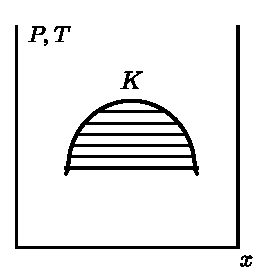
\includegraphics[width=6cm]{fig20.pdf}\\[0.3em]{\small 图 20}\end{minipage}\par\nopagebreak

由图20可以看出，在临界点附近存在两相彼此处于平衡的状态，这两相可以有任意接近的浓度 $x$ 和 $x+\delta x$.对于这样的两相，平衡条件具有形式
\begin{equation*}
  \mu(P,T,x)=\mu(P,T,x+\delta x),
\end{equation*}
式中 $\mu$ 是混合物中一种组分的化学势.由此可以看出（参看§83）：在临界点必须满足条件
\begin{equation}
  \left(\frac{\partial\mu}{\partial x}\right)_{P,T}=0.
\end{equation}
这个条件等同于条件(96.8)；因此临界点的这两种定义（这里的和§96中的）是等价的.必须注意：在(97.1)中，$\mu$ 所指的是混合物的两种组分中任一种的化学势.在(97.1)中取这一个还是另一个化学势所得到的两个条件实际上是等效的，这很容易证实，因为不论哪个化学势都是 $\varPhi$ 相对于相应粒子数的微商，而 $\varPhi$ 又是两种粒子数的一次齐次函数.

显然，临界点在平衡曲面上形成一条曲线.

在等浓度点附近，平衡曲线具有如图21所示的形状（或者是等浓度点 $K$ 为极小点的类似形状）.两条曲线在极大点（或极小点）相切.两条曲线之间的区域是两相分离的区域.在 $K$ 点，彼此处于平衡的两相的浓度变成相同，但是两相仍继续以分离的形式存在.这是因为：要从在 $K$ 点重合的两点中的任一点过渡到另一点，只能通过两相分离的区域来实现.像临界点一样，等浓度点也在平衡曲面上形成一条曲线.

\par\nopagebreak\noindent\begin{minipage}{\linewidth}\centering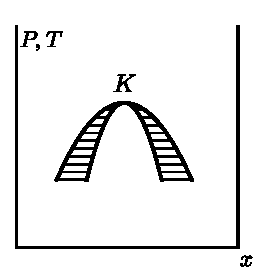
\includegraphics[width=6cm]{fig21.pdf}\\[0.3em]{\small 图 21}\end{minipage}\par\nopagebreak

现在我们来考虑平衡曲线在低浓度下的性质（这时混合物中一种物质比另一种少得多，即 $x$ 接近于0或1）.

在§89中已经证明：在低浓度下（即稀溶液的情形）溶液和纯物质的相平衡温度（在同一压强下）之差正比于两相浓度之差.对于在同一温度下的相平衡，压强之差也有同样的关系.除此以外，在§90中（也是对于低浓度的情形）还证明了两相中的浓度之比只与 $P$ 和 $T$ 有关，因而在 $x=0$ 附近，这个比值可以认为是常数.

从所有这些考虑可以直接得出结论：在低浓度下，平衡曲线具有如图22所示的形状，即由两条相交于纵坐标轴上的直线所构成（或者有直线朝上的类似形状）.在两条直线之间的区域是两相分离的区域.在这两条直线以上和以下的区域是一相和另一相的区域.

\par\nopagebreak\noindent\begin{minipage}{\linewidth}\centering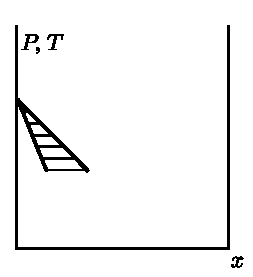
\includegraphics[width=5.5cm]{fig22.pdf}\\[0.3em]{\small 图 22}\end{minipage}\par\nopagebreak

\par\nopagebreak\noindent\begin{minipage}{\linewidth}\centering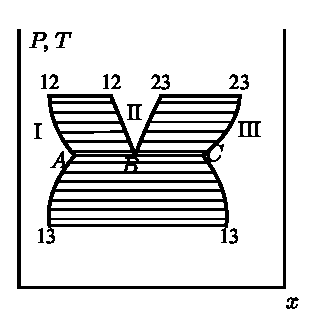
\includegraphics[width=5.5cm]{fig23.pdf}\\[0.3em]{\small 图 23}\end{minipage}\par\nopagebreak

在这一节的开头已经指出：由两种组分所组成的系统可以包含三个相互接触的相.在三相点附近平衡曲线的样子如图23所示.在平衡条件下，所有三相具有相同的压强和温度.因此，决定这三相的浓度的 $A$,$B$,$C$ 三点，位于与横坐标轴平行的同一直线上，$A$ 点所确定的是第一相在三相点的浓度，它是第一、二相间及第一、三相间的平衡曲线12和13的交点.类似地，$B$ 点是第一、二相间及第二、三相间的平衡曲线12和23的交点，而 $C$ 点是第二、三相间及第一、三相间的平衡曲线23和13的交点.自然，$A$,$B$,$C$ 三点是 $P=$ 常数或 $T=$ 常数的平面与平衡曲面上三条曲线的交点；在这三条曲线中，我们把相应于 $B$ 点的那一条曲线称为三相点线或三相线.Ⅰ，Ⅱ，Ⅲ三个区域各为第一相、第二相、第三相的单相态.在直线 $ABC$ 以下且在两条13曲线之间的区域，是分离成第一、第三两相的区域，而在两条12曲线之间以及在两条23曲线之间（且都在 $ABC$ 以上）的区域，各为分离成第一、第二两相及第二、第三两相的区域.区域Ⅱ显然必须整个位于 $ABC$ 以上（或整个位于 $ABC$ 以下）.一般来讲，曲线12,13,23以一定的角度在 $A$,$B$,$C$ 三点相交，而不是以光滑的方式互相过渡.当然，曲线12,13,23的方向不必像图23中所描绘的那样.重要的仅在于：曲线12和23以及曲线13必须位于直线 $ABC$ 的不同两侧.

如果把平衡曲面上上述这些特定曲线中的任一条投影到 $PT$ 平面上，那么这个投影把平面分成两部分.对于临界曲线，投影到这两部分之一的各点，是对应于两个不同单相的诸点以及对应于两相分离的诸点.投影到 $PT$ 平面的另一个部分上的诸点，则代表均匀的状态，同时在这些点中任何一点都不会发生两相分离.在图24中虚线表示临界曲线在 $PT$ 平面上的投影.字母 $a$,$b$ 代表两相.符号 $a-b$ 代表的是：投影到平面上这一部分的诸点是两个单相的状态以及两相彼此处于平衡的状态.符号 $ab$ 所代表的是 $a$ 和 $b$ 两相在临界点以上合并而成的一个单相.

\par\nopagebreak\noindent\begin{minipage}{\linewidth}\centering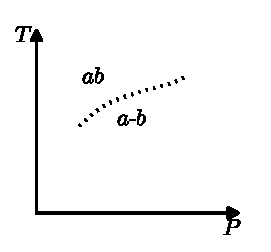
\includegraphics[width=6cm]{fig24.pdf}\\[0.3em]{\small 图 24}\end{minipage}\par\nopagebreak

类似地，三相线的投影也把 $PT$ 平面分成两部分.图25标示出哪些点投影到这两部分.符号 $a-b-c$ 表示：投影到这一部分的点代表 $a$,$b$,$c$ 三个单相的状态以及 $a$ 和 $b$ 或 $b$ 和 $c$ 两相分离的状态.

\par\nopagebreak\noindent\begin{minipage}{\linewidth}\centering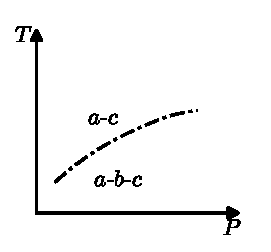
\includegraphics[width=6cm]{fig25.pdf}\\[0.3em]{\small 图 25}\end{minipage}\par\nopagebreak

图26表示等浓度点曲线的这种投影，图27表示纯物质（即 $x=0$ 或 $x=1$）的相平衡曲线；后者显然本来就在 $PT$ 平面上.图27上的字母 $b$ 表示：投影到 $PT$ 平面的这一部分的诸点对应于只有 $b$ 相的状态.我们假定在符号 $a-b$,$a-b-c$ 的字母序列中约定字母 $b$ 是浓度比 $a$ 大的相，而字母 $c$ 是浓度比 $b$ 大的相\footnote{为了避免误解，必须强调指出：对于等浓度线的情形（与三相线的情形不同），符号 $a-b-c$ 在某种意义下有随意性，这时 $a$ 和 $c$ 两个字母所代表的状态实际上并不是两个不同的相，因为它们永远都不会以相互接触的方式同时存在.}.

\par\nopagebreak\noindent\begin{minipage}{\linewidth}\centering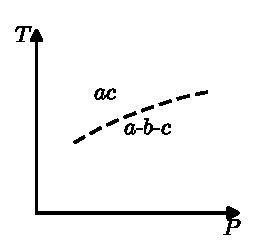
\includegraphics[width=6cm]{fig26.pdf}\\[0.3em]{\small 图 26}\end{minipage}\par\nopagebreak

\par\nopagebreak\noindent\begin{minipage}{\linewidth}\centering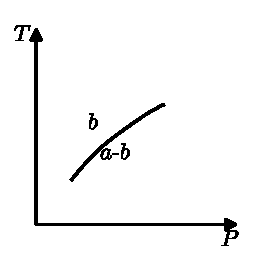
\includegraphics[width=6cm]{fig27.pdf}\\[0.3em]{\small 图 27}\end{minipage}\par\nopagebreak

必须注意：平衡曲线的这四种类型的特殊点（三相点、等浓度点、临界点和纯物质点）是平衡曲线的四种可能类型的极大（或极小）.

如果这些相中的任一相总是（不论 $P$ 和 $T$ 的值）具有同一个确定的组成，则平衡曲线在上述这些特殊点附近就变得稍为简单一些.这样的相是两种组分的化合物，或者是纯物质相即总有浓度 $x=0$（或 $x=1$）.

我们来讨论当成分不变的相存在时与之对应的平衡曲线在其端点附近的形状.显然，这样的点必须是平衡曲线的极大点或极小点，因而也就是在本节中所讨论过的各种类型的点.

如果成分不变的相是浓度 $x=0$ 的纯物质相，那么与它对应的线就同 $P$ 或 $T$ 轴重合，并且终止在如图28所示类型的点上.这个图描绘了平衡曲线在这种点附近的形状；图22中两条直线之一同纵坐标轴重合.

如果一相是成分确定的化合物，那么在等浓度点附近平衡曲线具有如图29所示的形状，即图21中的内部区域变成一条竖线.在它两侧的阴影区域是两相分离的区域，其中一相就是成分由这条直线所确定的化合物.在极大点曲线没有如图21所示的破洞.

类似地，在三相点附近平衡曲线具有如图30所示的形状.化合物的相由一条竖线表示，图23中的区域Ⅱ在这里退化为这条线.

\par\nopagebreak\noindent\begin{minipage}{\linewidth}\centering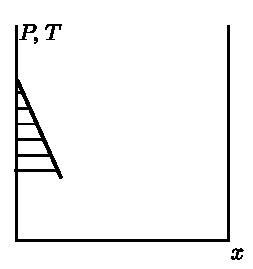
\includegraphics[width=5.5cm]{fig28.pdf}\\[0.3em]{\small 图 28}\end{minipage}\par\nopagebreak

\par\nopagebreak\noindent\begin{minipage}{\linewidth}\centering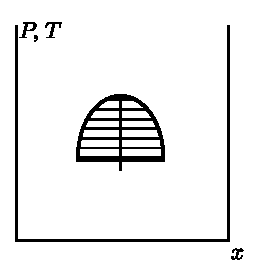
\includegraphics[width=5.5cm]{fig29.pdf}\\[0.3em]{\small 图 29}\end{minipage}\par\nopagebreak

\par\nopagebreak\noindent\begin{minipage}{\linewidth}\centering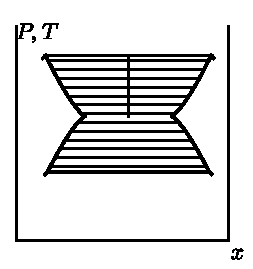
\includegraphics[width=5.5cm]{fig30.pdf}\\[0.3em]{\small 图 30}\end{minipage}\par\nopagebreak

\section{相图举例}

在这一节中我们要列举平衡曲线的基本类型；和上节不同，我们现在不仅在特殊点附近而且也在整体上考察它们的形状.这些曲线（也称为相图）可能具有各种各样的形状，但是在大多数情况下，它们可归于下面所讨论的类型之一，或者是由其中几种类型组合而成.在所有的相图上，凡是阴影区域都表示两相分离的区域；而无阴影的区域表示均匀状态的区域.两相分离区域的边界曲线与水平线的交点确定（在给定的 $P$ 和 $T$ 下）分离的两相的成分.同时，两相的相对量由§81中提到的“杠杆定则”来决定.

为了确定起见，我们在下面所讨论的都是 $Tx$ 图；如果用 $P$，$x$ 作为坐标，也可能有同样类型的相图.横坐标轴表示浓度 $x$，其变化范围在0到1之间.

1. 存在两相；每一相都可以具有任何浓度（即两相中的两种组分可以按任意比例混合）.在最简单的情形下，曲线没有任何极大值或极小值（除了相当于纯物质的点以外），这种相图的形式如图31所示（所谓“雪茄型”）.

\par\nopagebreak\noindent\begin{minipage}{\linewidth}\centering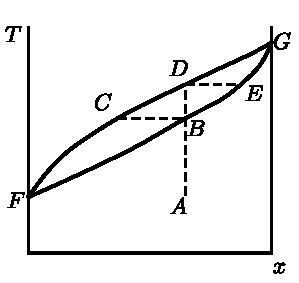
\includegraphics[width=6cm]{fig31.pdf}\\[0.3em]{\small 图 31}\end{minipage}\par\nopagebreak

例如，设其中一相是液体（雪茄以下的区域），而另一相是蒸气（雪茄以上的区域）；在这种情形下，雪茄的上面一根曲线称为凝聚曲线，下面一根曲线称为沸点曲线\footnote{液体混合物的沸腾与凝聚的规律由康诺瓦洛夫（Д.~П.~Коновалов, 1884）建立.}.

如果加热成分一定的液体混合物，那么在（对应于给定浓度的）竖线 $AD$ 同雪茄下曲线的交点（点 $B$）所确定的温度下，液体开始沸腾.这时沸腾出来的蒸气，其成分由点 $C$ 决定，就是说其浓度比液体低.剩下液体的浓度显然将提高，因而，它的沸点也将相应地提高.继续加热时，代表液相状态的点沿着下曲线向上移动，而代表沸腾出来的蒸气的点沿着上曲线向上移动.沸腾在什么温度结束，取决于过程如何进行.如果沸腾是在封闭的容器中进行，以至于沸腾出来的全部蒸气始终保持同液体接触，那么显然液体全部沸腾完毕的温度，就是蒸气的浓度达到液体起始浓度（点 $D$）的那个温度.因此，在这种情况下，沸腾开始和结束的温度分别决定于竖线 $AD$ 与雪茄的下和上曲线的交点.如果让沸腾出来的蒸气不断跑掉（在开放的容器中沸腾），则在每一时刻与液体处于平衡的都只是刚刚沸腾出来的蒸气.显然，在这种情形下，沸腾直至纯物质的沸点 $G$ 才结束，在这一点，液体和蒸气的成分一样.蒸气凝聚成液体也是以类似的方式进行的.

如果两相是液体（雪茄上方）和固体（雪茄下方），所发生的情况也完全相似.

2. 两种组分在两相中可以按任意比例混合（同上例），但是具有等浓度点.这种情形的相图具有如图32所示的形式（或具有极小值的类似形式）.在等浓度点，两条曲线具有极大值（或极小值），并且彼此相切.

\par\nopagebreak\noindent\begin{minipage}{\linewidth}\centering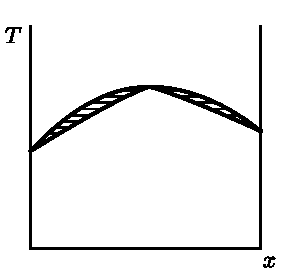
\includegraphics[width=6cm]{fig32.pdf}\\[0.3em]{\small 图 32}\end{minipage}\par\nopagebreak

从一相转变到另一相的相变过程，同上例描述的情况类似，不同之处只在于：（只要一相不断移去，如液体在开放容器中沸腾，）过程既可以在纯物质点，也可以在等浓度点结束.当成分正好相当于这一点时，整个过程始终在同一温度下发生\footnote{相应于等浓度点的混合物也称为\textbf{共沸混合物}.}.

3. 存在液体和气体两相，在这两相中两种组分可以按任意比例混合，并且具有临界点，相图如图33所示（$K$ 是临界点）.曲线右侧的区域相当于液态，左侧的区域相当于气态.但是应当提醒一下：在有临界点存在的情况下，只有当两相同时处于相互平衡时，才能够严格地区分液相和气相.

这种类型的相图导致下述的特殊现象.如果在封闭容器中加热液体，其成分由（通过点 $K$ 右侧的）直线 $AC$ 表示，那么在沸腾开始（在点 $B$）以后，随着加热的继续，蒸气量将逐渐增加，但是从某一时刻起，又开始减少，直到点 $C$ 蒸气完全消失（所谓逆行凝聚）.

\par\nopagebreak\noindent\begin{minipage}{\linewidth}\centering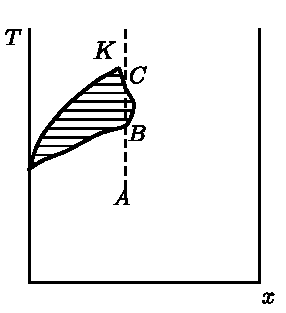
\includegraphics[width=7cm]{fig33.pdf}\\[0.3em]{\small 图 33}\end{minipage}\par\nopagebreak

4. 两种液体可以混合，但不能按任意比例.相图如图34所示.在高于临界点 $K$ 的温度下，两种组分可以按任意比例混合.低于这个温度，两种组分不能按由阴影区域内诸点所代表的比例来混合.在阴影区域内，液体分离成两相——两种液体混合物（两种溶液），它们的浓度决定于相应的水平线与平衡曲线的交点.类似的相图也有可能，包括其中点 $K$ 是极小点，或者有两个临界点一上一下，以至于两相分离（两种溶液）的区域被限制在一封闭曲线内.

\par\nopagebreak\noindent\begin{minipage}{\linewidth}\centering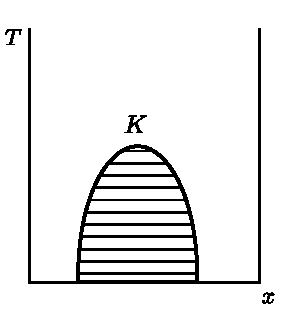
\includegraphics[width=6.5cm]{fig34.pdf}\\[0.3em]{\small 图 34}\end{minipage}\par\nopagebreak

5. 在液态（或气态）中两种组分可以按任意比例混合，而在固态（或液态）中不能按任意比例混合（有限互溶）.在这种情形下，存在着三相点.三相点的温度可能低于两种纯组分的相平衡温度（点 $A$ 和点 $C$），也可能介乎其间，（显然不可能高于它们，因为已经假设在高温相中两种组分可以任意混合，）相图的形式分别如图35和图36所示.不妨设具有无限互溶的一相为液体，而有限互溶的相为固体.在曲线 $ABC$（图35）或 $ADC$（图36）以上的区域是液态区；在曲线 $ADF$ 和 $CEG$（图35）或 $ABF$ 和 $CEG$（图36）两侧的区域是均匀固相（固溶体）的区域.在三相点（其温度决定于直线 $DBE$），液相和不同浓度的两种固溶体处于平衡.图35中的点 $B$ 称为共晶点.如果液体混合物具有相当于这一点的浓度，那么它的凝固完全保持同一浓度（而在其它的浓度下凝固出来的固体混合物，与液体有不同的浓度）.区域 $ADB$ 和 $CBE$（图35）以及区域 $ADB$ 和 $CDE$（图36）是分离成液相和一种固相的区域；区域 $DEGF$（图35）和 $BEGF$（图36）是分离成两种固相的区域.

如果在图35型的相图的情形下，两种组分在固态根本不能混合，那么相图就具有如图37所示的形式.在直线 $ABC$ 以上的阴影区域内，混合液体相和一种纯组分的固相处于平衡；在直线 $ABC$ 以下的阴影区域内，两种纯物质固相处于平衡.当降低液体混合物的温度时，从液体混合物中凝固出这种或那种纯组分，究竟是哪一种，取决于液体的浓度是在共晶点的右侧还是左侧.随着温度的继续降低，液体的成分沿着曲线 $DB$ 或 $EB$ 而变化，直到在共晶点 $B$ 液体全部凝固.

\par\nopagebreak\noindent\begin{minipage}{\linewidth}\centering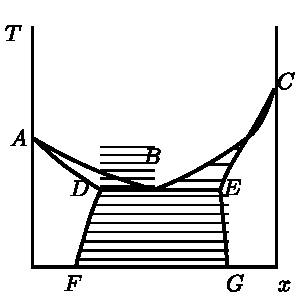
\includegraphics[width=7cm]{fig35.pdf}\\[0.3em]{\small 图 35}\end{minipage}\par\nopagebreak

\par\nopagebreak\noindent\begin{minipage}{\linewidth}\centering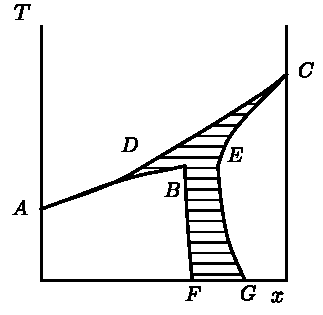
\includegraphics[width=7cm]{fig36.pdf}\\[0.3em]{\small 图 36}\end{minipage}\par\nopagebreak

\par\nopagebreak\noindent\begin{minipage}{\linewidth}\centering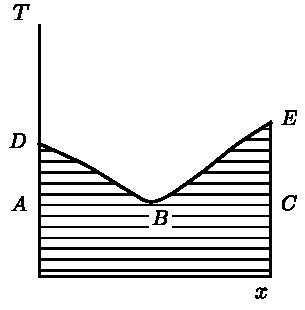
\includegraphics[width=7cm]{fig37.pdf}\\[0.3em]{\small 图 37}\end{minipage}\par\nopagebreak

6. 两种组分在液态可以按任意比例混合，而在固态根本不能混合，但形成成分固定的化合物.相图如图38所示.直线 $DE$ 决定化合物的成分.这时，有两个三相点 $B$ 和 $G$，在那里液相、固态化合物和一种纯组分固相处于平衡.位于 $B$ 和 $G$ 两点之间的是等浓度点 $D$（参看图29）.很容易看出相分离发生在哪里以及分离成什么相：在区域 $DBE$ 内，分离成液相和固态化合物，在直线 $CBE$ 以下，分离成化合物和一种纯组分的固态，等等.液体的凝固结束在共晶点之一 $G$ 或 $B$ 处，这取决于液体的浓度是在直线 $DE$ 的右侧还是左侧.

7. 两种组分在液态中可以按任意比例混合，在固态中则根本不能混合而是形成化合物，但是这种化合物在开始熔化以前的某个温度就已经分解了.确定这种化合物的成分的直线，不能像前一种情形那样终止在等浓度点，因为它不能达到熔点.因此，它可以终止于一个如§97中图30所示类型的三相点（图39上的点 $A$）.图39表示出这时相图的可能形式，不难看出在图中阴影区域内哪些点出现哪些相的分离.

8. 两种组分在固态中完全不能混合，在液态中也不能按任意比例混合.在这种情形有两个三相点，在那里液体与两种固态纯组分彼此处于平衡（图40中的点 $B$），或者一种纯组分与两种浓度不同的混合液相彼此处于平衡（点 $D$）.在曲线 $ABC$ 和曲线 $DE$ 以上的两个没有阴影的区域表示两种浓度不同的液态；直线 $CD$ 以上的阴影区域表示分离成这两种液相的区域；区域 $DEF$ 表示分离成液体和一种固态纯组分的区域；等等.

\par\nopagebreak\noindent\begin{minipage}{\linewidth}\centering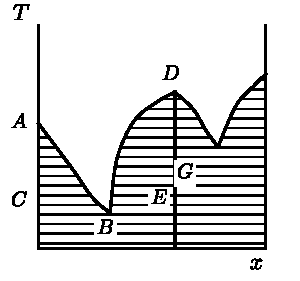
\includegraphics[width=6cm]{fig38.pdf}\\[0.3em]{\small 图 38}\end{minipage}\par\nopagebreak

\par\nopagebreak\noindent\begin{minipage}{\linewidth}\centering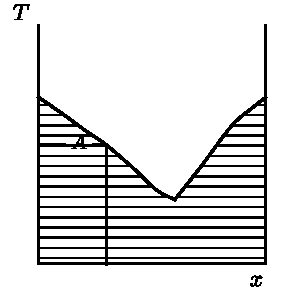
\includegraphics[width=6cm]{fig39.pdf}\\[0.3em]{\small 图 39}\end{minipage}\par\nopagebreak

\par\nopagebreak\noindent\begin{minipage}{\linewidth}\centering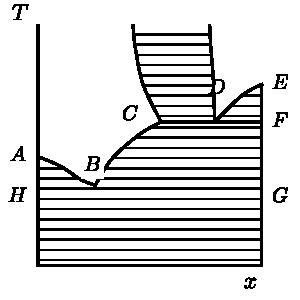
\includegraphics[width=6cm]{fig40.pdf}\\[0.3em]{\small 图 40}\end{minipage}\par\nopagebreak

\section{平衡曲面的特征曲线的相交}

在§97中所考虑的四种类型的曲线（临界线、三相线、等浓度线和纯物质线）都在同一个曲面（平衡曲面）上.因此一般来讲，它们彼此相交.我们来描述这些曲线交点的一些性质.

可以证明，两条临界线不可能彼此相交，两条等浓度线也不可能相交.对于这些结论，我们不准备在这里证明.

我们现在来列举其余的交点的性质（仍旧不作证明）.所有这些性质几乎都可以直接从§97中所讨论的平衡曲线的普遍性质引申出来.我们将图示上述曲线在 $PT$ 平面上的投影（参看§97）.它们的形状自然是随意取的.各处将用点线代表临界线，实线代表纯物质的相平衡线，虚线代表等浓度线，点划线代表三相线.字母与§97的图24—图27中的有相同意义.

临界线和纯物质线终止在它们的交点上（图41a）.临界线和三相线也是在它们相交时终止（图41b）.纯物质线同等浓度线相交时，只是后者终止了（图41c）.在这种情形下，两条曲线在交点处彼此相切.等浓度线相交于临界线（图41d）或三相线（图41e）时，情况相同.在这两种情形下，都是等浓度线终止在交点，并且两条曲线在交点彼此相切.

\par\nopagebreak\noindent\begin{minipage}{\linewidth}\centering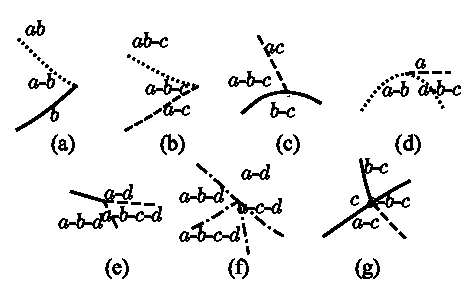
\includegraphics[width=10cm]{fig41.pdf}\\[0.3em]{\small 图 41}\end{minipage}\par\nopagebreak

三相线的交点（图41f）是四相点，即四相在这一点相互平衡.四条三相线在这点相遇，每条各自对应于四相中每三相的相互平衡.

最后，一条纯物质线和一条三相线的交点（图41g），显然应当是该三相线同时与所有三条纯物质的相平衡线（各自对应于纯物质的三相中每两相的相互平衡）之间的交点.

\section{气体和液体}

我们现在来更详细地考虑由两种组分所构成的液相和气相的平衡.

在温度足够高（$T$ 与分子的平均相互作用能相比很大）时，所有的物质都可以按任意比例混合.从另一方面来讲，在这样的温度下物质变成气体，因此可以说：在气相中一切物质都具有无限的互溶度.（其实，当存在临界线时，液体与气体之间的区别在某种意义下已成为一种约定，而上述说法也是如此.）

至于在液态中，有些物质可以按任意比例混合，另一些则只在一定的比例范围内混合（有限互溶的液体）.

对于两种组分在两相中都可按任意比例混合的前一种情形，这时相图中没有三相点，因为系统不可能由比两相更多的相来构成（所有的液态都是一相，所有的气态也都是一相）.我们来考虑平衡曲面的特征曲线在 $PT$ 平面上的投影.我们有两条纯物质的相平衡曲线（即两相中的浓度同为 $x=0$ 和 $x=1$ 的两条曲线）.这两条曲线中的一条本身就在 $PT$ 平面上，另一条则在与 $PT$ 平面平行的平面上，因此它的投影与它本身完全一样.每一条曲线都终止在某一点，这一点就是相应纯物质的相临界点，临界线从这样两点中的一点开始而在另一点终止（临界线和纯物质线二者都终止在它们的交点上；参看§99）.因此，所有这些曲线在 $PT$ 平面上的投影具有如图42所示的形式（记号与§97，§99中的完全相同）.字母 $g$ 和 $l$ 的意义与§97，§99的各图中所用的字母 $a$,$b$,$c$ 意义相同；$g$ 代表气体，$l$ 代表液体；投影到区域 $g$ 和 $l$ 中的分别为气态和液态；投影到区域 $g-l$ 中的是气态和液态，以及气态和液态分离的诸状态；在临界线以上，液体和气体的区别消失.

如果除此以外还有等浓度线，那么在 $PT$ 平面上的投影具有如图43所示的形式.等浓度线投影位于自坐标原点出发的线 $OB$ 以上（如图43所示），或者位于 $OC$ 以下，而不在其间.只有 $A$,$B$,$C$ 三点是这几条曲线的交点.点 $D$ 并不相当于纯物质线同临界线的实际交点，而只在投影上存在.图上的字母 $l_1$ 和 $l_2$ 代表浓度不同的液相.在等浓度线以上只能存在一种液相.

\par\nopagebreak\noindent\begin{minipage}{\linewidth}\centering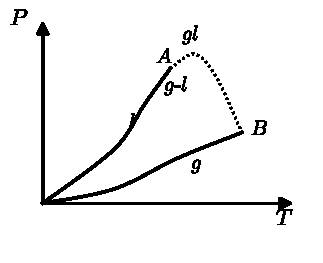
\includegraphics[width=6.5cm]{fig42.pdf}\\[0.3em]{\small 图 42}\end{minipage}\par\nopagebreak

\par\nopagebreak\noindent\begin{minipage}{\linewidth}\centering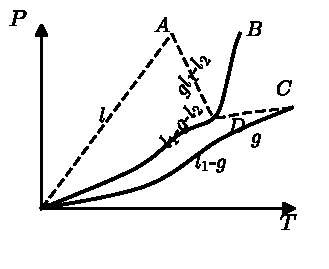
\includegraphics[width=6.5cm]{fig43.pdf}\\[0.3em]{\small 图 43}\end{minipage}\par\nopagebreak

用不同温度（或压强）的平面去截割平衡曲面将得到相应的相图，考察这样的相图可以使特定曲线在 $PT$ 平面上的投影的所有上述性质变得明显.例如，对应于压强在图42中的点 $B$ 以下以及在点 $A$ 和点 $B$ 之间的截面图，分别给出如图31和33所示的相图.图44中所表示的是图43在一系列温度下的截面图（$T_A$,$T_B$,$T_C$ 各为相当于 $A$,$B$,$C$ 各点的温度）：两相分离的区域在等浓度点发生“断裂”，结果形成两个临界点；随着温度的升高，两块阴影区域各向两纵坐标轴上的一点收缩，首先是一块、然后是另一块逐渐消失.图45上表示的是这同一情形在一系列压强下的截面图.

\par\nopagebreak\noindent\begin{minipage}{\linewidth}\centering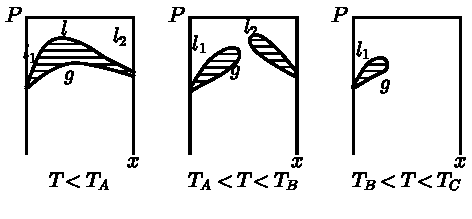
\includegraphics[width=10cm]{fig44.pdf}\\[0.3em]{\small 图 44}\end{minipage}\par\nopagebreak

\par\nopagebreak\noindent\begin{minipage}{\linewidth}\centering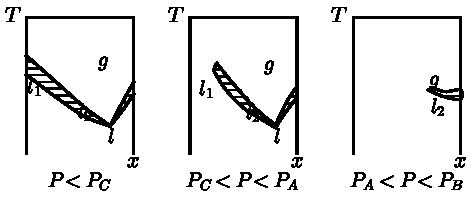
\includegraphics[width=9.5cm]{fig45.pdf}\\[0.3em]{\small 图 45}\end{minipage}\par\nopagebreak

如果两种组分在液态中的互溶度是有限的，那么有三相线存在.这条曲线终止在某一点，而与从该点开始的临界线相接.图46和图47中所表示的是在这种情形下可能发生的两种本质上不同类型的 $PT$ 投影图.它们的区别在于：三相线的投影在图46中是通过两条纯物质线的上方；而在图47中是通过它们两者之间（三相线的投影不可能通过两条纯物质线的下方，因为两种组分在气态中可以按任意比例混合）.在这两种情形中，每一种情形都有两条临界线，其中一条的趋向是朝着压强增大的方向.

\par\nopagebreak\noindent\begin{minipage}{\linewidth}\centering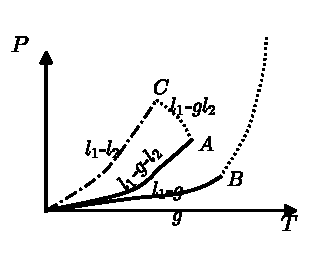
\includegraphics[width=6.5cm]{fig46.pdf}\\[0.3em]{\small 图 46}\end{minipage}\par\nopagebreak

\par\nopagebreak\noindent\begin{minipage}{\linewidth}\centering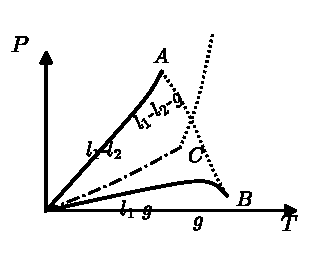
\includegraphics[width=6.5cm]{fig47.pdf}\\[0.3em]{\small 图 47}\end{minipage}\par\nopagebreak

对于图46所示的情形，顺序的几个 $Px$ 平面和 $Tx$ 平面截面图，如图48和图49所示.

\par\nopagebreak\noindent\begin{minipage}{\linewidth}\centering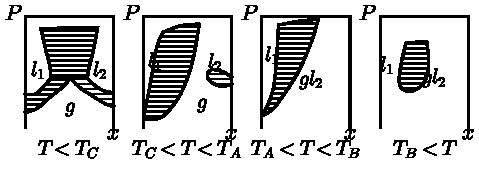
\includegraphics[width=9.5cm]{fig48.pdf}\\[0.3em]{\small 图 48}\end{minipage}\par\nopagebreak

\par\nopagebreak\noindent\begin{minipage}{\linewidth}\centering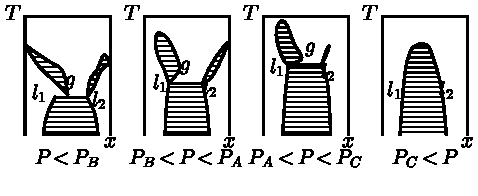
\includegraphics[width=10cm]{fig49.pdf}\\[0.3em]{\small 图 49}\end{minipage}\par\nopagebreak

最后必须强调的是：在这一节中所考虑的 $PT$ 图例子，只是液相和气相之间相互平衡的最典型例子，并没有把理论上所有可能的类型概括无遗.
